\nonstopmode
%%*****************************************************************************
%% Copyright (c) 2008-2010 Gerd Neugebauer
%%
%% Permission is granted to copy, distribute and/or modify this document
%% under the terms of the GNU Free Documentation License, Version 1.2
%% or any later version published by the Free Software Foundation;
%% with no Invariant Sections, no Front-Cover Texts, and no Back-Cover Texts.
%%
%%*****************************************************************************
%% $Id$
%%*****************************************************************************
%% Author: Gerd Neugebauer
%%-----------------------------------------------------------------------------
\documentclass%
    [final]%
    {extex-doc}

\def\Version{0.1}

\title{Reference Manual}
\author{Gerd Neugebauer}

\usepackage{dirlist}
\usepackage{iconmargin}
\usepackage{makeidx}

\newcommand\Arg[1]{\(\langle\){\tt\itshape #1}\(\rangle\)}
\newcommand\cli[1]{\texttt{#1}\index{#1@\texttt{#1}}}
\newcommand\CLi[1]{\texttt{-{}#1}\index{#1@\texttt{-{}#1}}}
\newcommand\CLI[1]{\texttt{-{}-#1}\index{#1@\texttt{-{}-#1}}}
\newcommand\Property[1]{\texttt{#1}\index{#1@\texttt{#1}}}
\newcommand\property[2]{\texttt{#1}\index{#2@\texttt{#1}}}
\newcommand\Env[1]{\texttt{#1}\index{#1@\texttt{#1}}}
\newcommand\File[1]{\texttt{#1}\index{#1@\textsf{#1}}}
\newcommand\Prog[1]{\texttt{#1}\index{#1}}
\newcommand\Mode[1]{\texttt{#1}\index{#1}}
\newcommand\macro[1]{\texttt{\char`\\ #1}\index{#1@\texttt{\char`\\ #1}}}
\newcommand\Macro[1]{\texttt{\char`\\ #1}}
\newcommand\Var[1]{\texttt{#1}\index{#1}}
\newcommand\Class[1]{\texttt{#1}\index{Class!#1}}
\newcommand\ClassIndex[1]{\index{Class!#1}}
\newcommand\Method[1]{\texttt{#1}\index{Method!#1()}}
\newcommand\MethodIndex[1]{\index{Method!#1()}}


\newcommand\tag[1]{%
    \ensuremath{\langle\textit{#1\index{#1@\protect\Tag{#1}}}\rangle%
    }}
\newcommand\Tag[1]{\texorpdfstring{%
    \ensuremath{\langle\textit{#1}\rangle}}{<#1>}}

\begingroup
  \catcode`\<=13
  \catcode`\|=13
  \gdef\SyntaxTag#1>{\tag{#1}}%
  \gdef\SyntaxConst#1|{\texttt{#1}}%
  \gdef\StartSyntax{%
    \let<\SyntaxTag
    \let|\SyntaxConst
    \let\IS\SyntaxDef
    \let\OR\SyntaxOr
    \let\+\SyntaxDefAdd
    \let\=\SyntaxDef
    \let\|\SyntaxOr
  }%
\endgroup
\newcommand\SyntaxDef{&\leftarrow&}
\newcommand\SyntaxDefAdd{&\leftarrow+&}
\newcommand\SyntaxOr{&|&}
\newenvironment{syntax}{%
  \catcode`\<=13
  \catcode`\|=13
  \StartSyntax
  \begin{eqnarray*}%
  }{%
  \end{eqnarray*}}

\def\n{\char`\\n}
\def\t{\char`\\t}

\providecommand\BibTeX{\texorpdfstring{%
    \textsc{Bib}\TeX}{BibTeX}}

\makeindex

\begin{document}%%%%%%%%%%%%%%%%%%%%%%%%%%%%%%%%%%%%%%%%%%%%%%%%%%%%%%%%%%%%%%%

\begin{titlepage}
  \parindent=0pt
  \begin{center}
  \vspace*{1pt}
  \vfill
  \ExBibbox
  \vfill
  \textsf{\bfseries\Huge \csname@title\endcsname}
  \vfill
  \textsf{\Large Version \Version}
  \vfill
  \textsf{\large \csname@author\endcsname}
  \vfill
  \vfill
%\maketitle

  \begin{abstract}\parindent=0pt
    This document describes \ExBib. It explains how to get \ExBib\ up
    and running and which features \ExBib\ offers to you.

    The intended audience for this document are end users of a
    bibliography processor who want to use \ExBib\ on the command line or
    as plug-in replacement of \BibTeX.
  \end{abstract}
  \ifdraft
  \unitlength=1mm
  \begin{picture}(0,0)
    \put(-39,196){\makebox(0,0){%
        \scalebox{5}{%
          \rotatebox{45}{%
            \color{black}\textsf{\Huge\bfseries Draft}}}}}
    \put(-40,195.5){\makebox(0,0){%
        \scalebox{5}{%
          \rotatebox{45}{%
            \color{red}\textsf{\Huge\bfseries Draft}}}}}
  \end{picture}
  \fi
  \end{center}
\newpage
\footnotesize
\copyright\ 2008--2010 The \ExTeX\ Group and individual authors listed below 
\medskip

Permission is granted to copy, distribute and/or modify this document
under the terms of the GNU Free Documentation License, Version 1.2 or
any later version published by the Free Software Foundation. A copy of
the license is included in the section entitled
``\hyperref[license:LGPL]{GNU Free Documentation License}''. \bigskip

This product includes software developed by the Apache Software
Foundation (\url{http://www.apache.org/}).

\vfill

Gerd Neugebauer\\
Im Lerchelsb\"ohl 5\\
64521 Gro\ss-Gerau (Germany)
\smallskip

\href{mailto://gene@gerd-neugebauer.de}{gene@gerd-neugebauer.de}

\end{titlepage}

%------------------------------------------------------------------------------

\tableofcontents

%------------------------------------------------------------------------------

%%*****************************************************************************
%% $Id: bst-language.tex,v 0.00 2008/04/30 23:26:21 gene Exp $
%%*****************************************************************************
%% Author: Gerd Neugebauer
%%-----------------------------------------------------------------------------

\chapter{Introduction}
%@author Gerd Neugebauer

\ExTeX\index{ExTeX@\ExTeX} aims at providing a high-quality
typesetting system. The development of \ExTeX\ has been inspired by
the experiences with \TeX\ \cite{knuth:texbook}. The focus lies on an
open design and a high degree of configurability.

A tight integration of several components is one of the possibilities
opened by \ExTeX. To work into this direction \ExBib\ has been
implemented. It is a plug-in replacement for
\BibTeX~0.99c\index{BibTeX 0.99c@\BibTeX~0.99c}\cite{btxdoc,btxhak}
or \BibTeX~8\index{BibTeX 8@\BibTeX~8}.

\begin{figure}[hb]
  \centering
  %%*****************************************************************************
%% $Id$
%%*****************************************************************************
%% Author: Gerd Neugebauer
%%-----------------------------------------------------------------------------
\begingroup\small
\def\processor(#1)#2{%
  \begin{scope}[shift={(#1)}]
    \draw[thick,color=white!80!gray,fill==white!70!gray]
    (1,-0.5) rectangle (9,4.5);
    \shade[top color=white!90!green,bottom color=white!60!green,draw=green!40!black,thick]
    (0.5,0) rectangle (8.5,5);
    \draw (4.5,2.5) node{#2};
    \shade[top color=white!90!green,bottom color=white!60!green,draw=green!40!black,thick]
    (0,1) rectangle (1,2);
    \shade[top color=white!90!green,bottom color=white!60!green,draw=green!40!black,thick]
    (0,3) rectangle (1,4);
  \end{scope}
}
\def\data(#1)#2{%
  \begin{scope}[shift={(#1)}]
    \draw[thick,color=white!80!gray,fill==white!70!gray]
    (0.3,-.3) -- (5.3,-.3) -- (5.3,1.7) -- (4.3,2.7) -- (0.3,2.7) -- cycle;
    \shade[top color=white!90!yellow,bottom color=white!60!yellow,draw=red!40!black,thick]
    (0,0) -- (5,0) -- (5,2) -- (4,3) -- (0,3) -- cycle;
    \draw (2.5,1.5) node{#2};
  \end{scope}
}
\def\datas(#1)#2{%
  \begin{scope}[shift={(#1)}]
    \draw[thick,color=white!80!gray,fill==white!70!gray]
    (0.3,-.3) -- (5.3,-.3) -- (5.3,1.7) -- (4.3,2.7) -- (0.3,2.7) -- cycle;
    \begin{scope}[shift={(.15,.15)}]
      \draw[thick,color=white!80!gray,fill==white!70!gray]
      (0.3,-.3) -- (5.3,-.3) -- (5.3,1.7) -- (4.3,2.7) -- (0.3,2.7) -- cycle;
    \end{scope}
    \begin{scope}[shift={(.1,.1)}]
      \draw[thick,color=white!80!gray,fill==white!70!gray]
      (0.3,-.3) -- (5.3,-.3) -- (5.3,1.7) -- (4.3,2.7) -- (0.3,2.7) -- cycle;
    \end{scope}
    \begin{scope}[shift={(.05,.05)}]
      \draw[thick,color=white!80!gray,fill==white!70!gray]
      (0.3,-.3) -- (5.3,-.3) -- (5.3,1.7) -- (4.3,2.7) -- (0.3,2.7) -- cycle;
    \end{scope}
    \begin{scope}[shift={(.3,.3)}]
      \shade[top color=white!90!yellow,bottom color=white!60!yellow,draw=red!40!black,thick]
      (0,0) -- (5,0) -- (5,2) -- (4,3) -- (0,3) -- cycle;
    \end{scope}
    \begin{scope}[shift={(.2,.2)}]
      \shade[top color=white!90!yellow,bottom color=white!60!yellow,draw=red!40!black,thick]
      (0,0) -- (5,0) -- (5,2) -- (4,3) -- (0,3) -- cycle;
    \end{scope}
    \begin{scope}[shift={(.1,.1)}]
      \shade[top color=white!90!yellow,bottom color=white!60!yellow,draw=red!40!black,thick]
      (0,0) -- (5,0) -- (5,2) -- (4,3) -- (0,3) -- cycle;
    \end{scope}
    \shade[top color=white!90!yellow,bottom color=white!60!yellow,draw=red!40!black,thick]
    (0,0) -- (5,0) -- (5,2) -- (4,3) -- (0,3) -- cycle;
    \draw (2.5,1.5) node{#2};
  \end{scope}
}
\def\arrow(#1)#2#3{%
  \begin{scope}[shift={(#1)}#3,scale=.5]
    \begin{scope}[shift={(#2)}]
      \draw[thick,color=white!80!gray,fill==white!70!gray]
      (0,1) -- (5,1) -- (5,0) -- (6,2) -- (5,4) -- (5,3) -- (0,3) -- cycle;
    \end{scope}
    \shade[top color=white!90!gray,bottom color=white!60!gray,draw=gray!40!black,thick]
    (0,1) -- (5,1) -- (5,0) -- (6,2) -- (5,4) -- (5,3) -- (0,3) -- cycle;
  \end{scope}
}
%
\begin{tikzpicture}[scale=.35]\sf
  \processor(10,30){Text Processor}

  \arrow(10.5,29){.3,.3}{,rotate=270}
  \datas(9,22){file.aux}
  \arrow(10.5,21){.3,.3}{,rotate=270}

  \processor(10,12){\ExBib}
  \arrow(19.5,13.5){.3,-.3}{}
  \data(23.5,13){file.blg}

  \arrow(18.5,18){-.3,-.3}{,rotate=90}
  \data(15,22){file.bbl}
  \arrow(18.5,26){-.3,-.3}{,rotate=90}

  \arrow(6,13.5){.3,-.3}{}
  \datas(0,13){*.bib}

  \arrow(12.5,8){-.3,-.3}{,rotate=90}
  \datas(9,4){*.bst}

  \arrow(18.5,8){-.3,-.3}{,rotate=90}
  \data(15,4){*.csf}

  \arrow(23,10){-.3,-.3}{,rotate=135}
  \datas(21,5){Config}

\end{tikzpicture}
\endgroup
\endinput
%
% Local Variables: 
% mode: latex
% TeX-master: nil
% End: 

  \caption{\ExBib\ and the Text Processor}%
  \label{fig:files}
\end{figure}
The principal interaction of a bibliography processor and a text
processor\index{text processor} has been defined by
\BibTeX\index{BibTeX@\BibTeX}. This is depicted in
figure~\ref{fig:files}. The underlying communication structure is file
based. This scheme is supported by \ExBib\ as well.

The main input from the text processor\index{text processor} is
transferred in the \texttt{aux} file. In \LaTeX\index{LaTeX@\LaTeX}
(cf. \cite{lamport:latex,goosens.mittelbach:latex.companion}) the
directive \macro{include} can be used to conditionally include parts
of a complete document. To make this work several \texttt{aux} files
are written -- one for each fragment. This \ExBib\ has to cope with
several \texttt{aux} files.

The \texttt{aux} files contain the information on the databases to be
used and the bib style. Accordingly the databases and the style are
read. As a result of the processing a formatted list of database
entries is produced in a \texttt{bbl} file. Additionally logging
information may be sent to a log file. The \texttt{bbl} file can be
read in by the text processor to include the entries into the
document. This completes the cycle.

One cycle may not be enough to resolve all citations. If the database
entries contain references (in form of \verb|\cite|
macros\index{cite@\verb/\cite/}). Then they can be resolved in a
second round. Unfortunately this may theoretically continue ad
infinitum. Practically spoken this has not been observed in real life.
Most of time one cycle or at most two of them are sufficient.


\section{Bibliography Processors -- a Short History}

\BibTeX\ is the well known bibliography processor in the \TeX\ world.
It has been written by Oren Patashnik\index{Patashnik, Oren} in 1983
to 1988. The foundations are older. \BibTeX\ refers in some aspects
back to Scribe\index{Scribe}.

The current release is \BibTeX~0.99c (\cite{btxdoc,btxhak}). The
development seems to be ended.\IM{0}

The long awaited release \BibTeX~1.0 should finalize the development
and include some additional features. Several papers have been published
(\cite{patashnik:bibtex1.0,patashnik:bibtex}) but a working version
has not been seen yet.\IM{1}

Since \BibTeX~0.99c has some deficiencies with respect to sorting and
character sets a rewrite in has been done by Niel
Kempson\index{Kempson, Niel} and Alejandro
Aguilar-Sierra\index{Aguilar-Sierra, Alejandro} around 1996. This is
\BibTeX~8. \BibTeX~8 uses internally 8-bit characters and provides
means to deal with different encodings.\IM{8}


ML\BibTeX\index{MLBibTeX@ML\BibTeX} is an attempt oif Jean-Marie
Hufflen\index{Hufflen, Jean-Marie} to rewrite \BibTeX\ and enhance ot
with features for multi-lingual processing.

\INCOMPLETE


\section{This Document}

This document is meant to be a reference document. It should contain
all information necessary to know. It is not meant to be a tutorial.
Thus do not expect tutorial type material in this document.


\section{Web Site}%
%@author Gerd Neugebauer

\begin{figure}[!ht]
  \centering
  \includegraphics[width=.5\textwidth]{img/www-extex-org}
  \caption{\texttt{www.extex.org}}
  \label{fig:www.exetex.org}
\end{figure}
There is a web site devoted to \ExTeX.\index{WWW}\index{Web Site} This
web site (see figure~\ref{fig:www.exetex.org}) can be reached via the
URL\index{www.extex.org}
\begin{quotation}
  \url{http://www.extex.org}
\end{quotation}


\section{Mailing Lists}
%@author Gerd Neugebauer

If you are ready to try \ExBib{} you might as well want to join a
mailing list to get in contact with the community.\index{mailing list}

\begin{quotation}
  \url{http://www.dante.de/listman/extex}
\end{quotation}


\section{Reporting Bugs}
%@author Gerd Neugebauer


If you find any bugs in \ExBib\ you can submit them 
%either 
via a HTML form.
% or via email. 
You can find the HTML form at
\begin{quotation}
  \url{http://www.extex.org/bugs}
\end{quotation}
%Emails containing the description can be sent to
%\begin{quotation}
%  \href{mailto:extex-bugs@dante.de}{extex-bugs@dante.de}
%\end{quotation}

Please include in your description 
\begin{itemize}
\item the source of a \emph{minimal} example showing the problem
\item the log file resulting from running this example
\item a description why you think that something went wrong and what
  the expected result would be
\item a description of the environment you are using (host
  architecture, operating system, Java version)
\end{itemize}

\endinput
%
% Local Variables: 
% mode: latex
% TeX-master: "exbib-users"
% End: 

%%*****************************************************************************
%% $Id: started.tex,v 0.00 2008/05/01 17:52:50 gene Exp $
%%*****************************************************************************
%% Author: Gerd Neugebauer
%%-----------------------------------------------------------------------------

\chapter{Getting Started}
%@author Gerd Neugebauer

In this chapter we describe the steps you can take to get \ExBib\ up
and running. We try to use as few as possible premises. Thus it should
be not too hard to get started.

\section{Prerequisites}
%@author Gerd Neugebauer

\subsection{Java}
%@author Gerd Neugebauer

You need to have Java 5\index{Java} or later installed on your
system. You can get Java for a several systems directly from
\url{java.sun.com}. Download and install it according to the
installation instructions for your environment.

To check that you have an appropriate Java on your path you can use
the command \texttt{java} with the argument \texttt{-version}. This
can be seen in the following example:

\lstset{morecomment=[l]{\#}}%
\begin{lstlisting}{morecomment=[l][keywordstyle]{>}}
# java -version
java version "1.5.0_04"
Java(TM) 2 Runtime Environment, Standard Edition (build 1.5.0_04-b05)
Java HotSpot(TM) Client VM (build 1.5.0_04-b05, mixed mode)
#
\end{lstlisting}


\subsection{TEXMF}
%@author Gerd Neugebauer

If you want to use more than the pure \ExBib\ engine, styles can be
inherited from a texmf tree\index{texmf}. \ExBib\ itself does not
contain a full texmf tree. It comes just with some rudimentary files
necessary for testing and getting started. Thus you should have
installed a texmf tree, e.g. from a \TeX Live\index{TeXlive@\TeX Live}
installation. This can be found on the
\href{http://www.ctan.org}{Comprehensive \TeX\ Archive Network
  (CTAN)}\index{CTAN}.

There is no need to install the texmf tree in a special place. You
have to tell \ExBib\ anyhow where it can be found. It is even possible
to work with several texmf trees.

One requirement for the texmf trees is that they have a file database
(\File{ls-R}). \ExBib\ can be configured to work without it, but then
\ExBib\ is deadly slow. Thus you do not really want to try this
alternative.


\section{Getting \ExBib}
%@author Gerd Neugebauer

\subsection{Getting the Installer}
%@author Gerd Neugebauer

The simplest way to get \ExBib\ up and running is to use the \ExBib\ 
installer. This installer\index{installer} is distributed as one file
\File{ExBib-setup.jar}. You can download it from

\begin{quotation}
  \url{http://www.extex.org/download/}
\end{quotation}

If you have got the installer there is no need for you to get the
sources as well. Nevertheless the soruces can be retrieved via
Subversion from
\begin{quotation}
  \url{https://svn.berlios.de/svnroot/repos/extex/trunk/ExBib}
\end{quotation}


\section{Installing \ExBib}\label{sec:install}
%@author Gerd Neugebauer

The installation of \ExBib\ works with the \ExBib\ installer. This
installer is named \File{ExBib-setup.jar}. You can start the installer
with the following command line:\index{installer}

\begin{lstlisting}{}
# java -jar ExTeX-setup.jar
\end{lstlisting}

On Windows\index{Windows} with a properly installed Java\index{Java}
you can also start the installer by double-clicking
\texttt{ExBib-setup.jar} in the Explorer\index{Explorer}. This might
work on other windowing systems as well.

\begin{figure}[!ht]
  \centering
  \includegraphics[width=.45\textwidth]{img/inst1}\hfill
  \includegraphics[width=.45\textwidth]{img/inst2}
  \caption{The Language Selection in the Installer}
  \label{fig:inst1}
\end{figure}
The installer provides a graphical user interface with a wizard
guiding you through the installation process. The first dialog is
shown in figure~\ref{fig:inst1}. As you can see you can select one of
several languages for the installation process. This selection just
effects the language used to communicate during the instanllation
process.  Currently the languages English and German are supported.
There might be some more at the time you are performing the
installation.\index{installer!language}\index{language!installer}

Note that the language selection covers the installer only. \ExBib\ 
can be run under different language environments as well. This is
controlled by a setting at run-time. Currently only an English and
a German language binding for \ExBib\ are provided.\index{language}

\begin{figure}[!ht]
  \centering
  \includegraphics[width=.45\textwidth]{img/inst3}
  \caption{Welcome to \ExBib}
  \label{fig:inst2}
\end{figure}

The next panel shows a welcome message showing what this installer is
about (see figure~\ref{fig:inst2}). Since you are reading this
document there is nothing new for you.

\begin{figure}[!ht]
  \centering
  \includegraphics[width=.45\textwidth]{img/inst4}
  \caption{Accepting the Licence}
  \label{fig:inst3}
\end{figure}

Now the license of \ExBib\ is presented (see figure~\ref{fig:inst3}).
It is there to remind you that there is something like a license. You
can not do everything with the software. But the limitations are very
minimalistic. Usually it should not really affect you -- especially
when you are migrating from \BibTeX.

Note that the license is the LGPL. In contrast to the GPL it does not
infect other software build from \ExBib\ or containing it.

\begin{figure}[!ht]
  \centering
  \includegraphics[width=.45\textwidth]{img/inst5}
  \caption{Selecting the Packages}
  \label{fig:inst4}
\end{figure}

Next the packages to be installed can be selected (see
figure~\ref{fig:inst4}). The core packages is needed in any case. Thus
it can not be deselected. The other packages can be freely choosen
from.

Whenever you select a package in the list a short discription of the
package is displayed.

\begin{figure}[!ht]
  \centering
  \includegraphics[width=.45\textwidth]{img/inst6}
  \caption{Selecting the Installation Directory}
  \label{fig:inst5}
\end{figure}

Finally the installation directory has to be selected (see
figure~\ref{fig:inst5}). The installation directory (see also
section~\ref{sec:inst.dir}) is the only directory the \ExBib\ 
installer creates files in. Usually is should be separate from other
directories. For instance the value \verb|C:\Program Files\ExBib| on
Windows or \verb|/opt/ExBib| on Unix are sensible values. Nevertheless
the installation can also be performed in your home directory if you
do not have writing permissions in the global directories.

This is the last decision you have to make.

\begin{figure}[!ht]
  \centering
  \includegraphics[width=.45\textwidth]{img/inst7}
  \caption{Progress of the Installation}
  \label{fig:inst6}
\end{figure}

Now the installation is performed. A progress panel is shown during
the installation (see figure~\ref{fig:inst6}). As a result the
installation directory is created and filled (see also
section~\ref{sec:inst.dir})

\begin{figure}[!ht]
  \centering
  \includegraphics[width=.45\textwidth]{img/inst8}
  \caption{Saving the Installation Settings}
  \label{fig:inst7}
\end{figure}

When the installation is completed you get the chance to save the
settings for unattended replay (see figure~\ref{fig:inst7}). See
section~\ref{sec:replay} for details.


Finally you have to make sure that the executables \Prog{exbib} or
\Prog{exbib.bat} are on your path for executables.\index{path} This
can be achieved by modifying the environment variable \verb|PATH| in a
Unix environment or setting \verb|path| in the system settings on
Windows.


\subsection{The Installation Directory}\label{sec:inst.dir}
%@author Gerd Neugebauer

During the installation you choose a directory where \ExBib\ lives.
This is called the installation directory. An example of the contents of the
installation directory can be seen in figure~\ref{fig:inst.dir}.

\begin{figure}[!ht]
  \centering
\begin{DirList}{200pt}{250pt}
  \TOPDIR(0,30){ExBib}
  \DIR(3,28)2{Uninstaller}
  \FILE(6,26)2{uninstaller.jar}
  \DIR(3,24){4.75}{bin}
  \FILE(6,22)2{exbib}
  \FILE(6,20){2.5}{exbib.bat}
  \FILE(6,18){2.5}{exbibutil}
  \FILE(6,16){2.5}{exbibutil.bat}
  \DIR(3,14){10.75}{doc}
  \FILE(6,12)2{exbib-manual.pdf}
  \DIR(3,10){4.75}{lib}
  \FILE(6,8){2}{ExBib-core.jar}
  \FILE(6,6){2.5}{ExBib-Main.jar}
  \FILE(6,4){2.5}{ExBib-styles.jar}
  \FILE(6,2){2.5}{ExTeX-resource.jar}
  \FILE(3,0){10.75}{LICENSE.txt}
\end{DirList}
  \caption{The Installation Directory}

  \label{fig:inst.dir}
\end{figure}

The directory \File{Uninstaller} contains the uninstaller. It can be
used to get rid of \ExBib\ -- even when I don't know why you should
want to. For details see section~\ref{sec:uninst}

The directory \File{bin} contains the binaries. This directory should
be put onto the path for executables. Note that currently all
executables are installed on any platform. On Windows the programs
without extension can be useful within the cygwin world. On Unix the
files with the extension \verb|.bat| can be simply ignored.

The directory \File{doc} contains documentation if the documentation
package has been selected during the installation.

The directory \File{lib} contains the libraries used by \ExBib.


\subsection{Replaying an Installation}\label{sec:replay}
%@author Gerd Neugebauer

Sometimes it is desirable to perform an installation on several
similar machines. This means that the answers to the questions in the
installer are the same. This process can be automated.

In figure~\ref{fig:inst7} you can see the last screen of the
installer. Here you have the possibility to select the button
``Generate an automatic installation script''. This produces an XML
file which can be passed to the installer to avoid the
dialogs.\index{installer}\index{installation script}

Suppose you have named the file \texttt{replay.xml} in the file
selector which pops up when the button has been pressed. Then you can
replay the installation with the following command invocation:

\begin{lstlisting}{}
# java -jar ExBib-setup.jar replay.xml
\end{lstlisting}

This supposes that the two files \File{ExTeX-setup.jar} and
\texttt{replay.xml} are in the current directory.

\subsection{Uninstalling \ExBib}\label{sec:uninst}
%@author Gerd Neugebauer

The files installed by the installer (see section~\ref{sec:install})
can be removed from the system. For this purpose an uninstaller is
provided in the subdirectory \File{Uninstaller} of the \ExBib\
installation directory. It is named \File{uninstaller.jar}. It can be
invoked by double clicking or invoking it on the command line as follows:

\begin{lstlisting}{}
# java -jar uninstaller.jar
\end{lstlisting}

\begin{figure}[!h]
  \centering
  \includegraphics[width=.45\textwidth]{img/uninst1}
  \caption{Confirming the Uninstallation}
  \label{fig:uninst1}
\end{figure}

When the uninstaller starts it asks for configmation (see
figure~\ref{fig:uninst1}). Nothing is changed before the confirmation
is given.

\begin{figure}[!h]
  \centering
  \includegraphics[width=.45\textwidth]{img/uninst2}
  \caption{The Uninstaller Finished}
  \label{fig:uninst2}
\end{figure}

The uninstaller shows a progress bar (see figure~\ref{fig:uninst2}).
When the uninstaller has finished its work all files and directories
installed with the installer have been removed. Modified and other
files are left untouched.

You can uninstall \ExBib\ by simply removing the installation
directory. But this is unsave since all local modification are lost as
well.

%%*****************************************************************************
%% $Id: cli-exbib.tex,v 0.00 2008/05/02 17:03:28 gene Exp $
%%*****************************************************************************
%% Author: Gerd Neugebauer
%%-----------------------------------------------------------------------------


%------------------------------------------------------------------------------
\section{Running \ExBib}
%@author Gerd Neugebauer

Currently \ExBib\ can be run from the command line. In this respect it
is more or less identical to \BibTeX\ and can be used as a plug-in
replacement. In addition the features of \BibTeX~8 are present as
well. The marks in the margin indicate where the different features
are coming from.

The exxecutable for \ExBib\ is called \Prog{exbib}. It is a wrapper
for the real program. It comes as shell script \Prog{exbib} and the
Windows batch script \Prog{exbib.bat}. After a successful installation
those scripts should be resent on your execution path.


\subsection{Command Line Parameters}
%@author Gerd Neugebauer

The invocation of the executable \Prog{exbib} can be controlled by
large number of command line arguments. Those command line arguments
are described in the following sections.

\subsubsection{The Aux File}

\begin{description}
\item[\Arg{file}]\ \\
  This parameter contains the aux file to read from. A file name may not
  start with minus sign. It has no default.
  \begin{lstlisting}{}
    # exbib doc.aux
    This is exbib, Version 0.1
  \end{lstlisting}
  
\item[\CLI{} \Arg{file}]
\item[\CLI{-} \Arg{file}]\ \\
  This parameter terminates the intercepts processing of arguments. The
  next argument -- if present -- is interpreted as input file. With
  this construction it is possible to process an input file which
  starts with the special character \verb|-|.
  \begin{lstlisting}{}
    # exbib -- doc.aux
    This is exbib, Version 0.1
  \end{lstlisting}

\end{description}

The file name given is used to determine the name of an aux file. This
means that it is either the name of an aux file or the base name which
is augmented by the extension \texttt{.aux} to find the aux file.

The main control information is taken from this aux file. This means
it contains the foloowing items:

\begin{itemize}
\item The database files to consult.
\item The citations to extract.
\item The bst to use for formatting.
\item References to other aux files to consult as well.
\end{itemize}

\subsubsection{Version Information and Help}

\begin{description}
\item[\CLI{-copying}]\ \\
  This command line option produces a copyright notice on the standard
  output stream and terminates the program afterwards.
  \begin{lstlisting}{}
# exbib --copying
                 GNU LESSER GENERAL PUBLIC LICENSE
                      Version 2.1, February 1999
Copyright (C) 1991, 1999 Free Software Foundation, Inc.
    59 Temple Place, Suite 330, Boston, MA  02111-1307  USA
Everyone is permitted to copy and distribute verbatim copies
of this license document, but changing it is not allowed.
[This is the first released version of the Lesser GPL.  It also counts
as the successor of the GNU Library Public License, version 2, hence
the version number 2.1.]
                           Preamble
 The licenses for most software are designed to take away your
freedom to share and change it.  By contrast, the GNU General Public
Licenses are intended to guarantee your freedom to share and change
free software--to make sure the software is free for all its users.
    ...
  \end{lstlisting}

\item[\CLI{h}]
\item[\CLI{?}]
\item[\CLI{-help}]\ \\
  This command line option produces a short usage description on the
  standard output stream and terminates the program afterwards.
  \begin{lstlisting}{}
# exbib --help
This is exbib, Version 0.1
Usage: exbib <options> file
The following options are supported:
        -[-] <file>
                Use this argument as file name -- even when it looks like an option.
        --trad[itional] | -7
                operate in the original 7-bit mode.
        --8[bit] | -8
                force 8-bit mode, no CS file used.
    ...
\end{lstlisting}
  
\item[\CLI{-release}]\ \\
  This command prints the release number to stdout and exits the
  program. This can be used to enable external programs to easily
  determine the version number of \ExBib.
\begin{lstlisting}{}
# exbib --release
0.1
#
\end{lstlisting}

\item[\CLI{-version}]\ \\
  This command line parameter forces that the version information is
  written to standard output and the program is
  terminated.\index{version} The version of \ExBib\ is shown. The
  following example shows a possible invocation and the resulting
  output:
\begin{lstlisting}{}
# exbib --version
This is exbib, Version 0.1
Copyright (C) 2002-2008 Gerd Neugebauer (mailto:gene@gerd-neugebauer.de).
There is NO warranty.  Redistribution of this software is
covered by the terms of the GNU Library General Public License.
For more information about these matters, use the command line
switch -copying.
#
\end{lstlisting}
\end{description}


\subsubsection{Internationalization}

\begin{description}
\item[\CLI{L} \Arg{lang}]
\item[\CLI{-language} \Arg{lang}]\ \\
  This command line option switches the language to the given
  language. The argument is a two-letter ISO code for a language. For
  instance the value \texttt{en} represents English and \texttt{de}
  represents German.

  The language is used to select the appropriate messages for logging
  and error messages. If the given language is not supported English
  is silently used as fallback.
\begin{lstlisting}{}
# exbib --language de --help
Dies ist exbib, Version 0.1
Copyright (C) 2002-2008 Gerd Neugebauer (mailto:gene@gerd-neugebauer.de).
There is NO warranty.  Redistribution of this software is
covered by the terms of the GNU Library General Public License.
For more information about these matters, use the command line
switch -copying.
#
\end{lstlisting}
\end{description}


\subsubsection{Configurations}
\index{configuration|(}

\ExBib\ is highly configurable. The whole system is assembled from
components at run time. The assembly is controlled from a set of
configuration files. There is one central configuration file which
acts as entry point.

\begin{description}
\item[\CLI{c} \Arg{config}]
\item[\CLI{-configuration} \Arg{config}]\ \\
  Set the configuration file to be used for assenbling \ExBib. The
  default is the configuration \texttt{exbib}.
\begin{lstlisting}{}
# exbib --configuration bibtex099 doc.aux
This is exbib, Version 0.1
...
\end{lstlisting}

\item[\CLI{-bibtex}]
\item[\CLI{-strict}]\ \\
  Use the configuration \texttt{bibtex099} for assembling \ExBib.
\begin{lstlisting}{}
# exbib --bibtex doc.aux
This is exbib, Version 0.1
...
\end{lstlisting}
\end{description}

The following configurations are present in the distribution.

\begin{description}
\item[exbib]\ \\
  This is the default configuration which includes all features
  described in this reference manual.
\item[bibtex099]\ \\
  This is the configuration for backward compatibility. It emulates
  the features of \BibTeX~0.99c as closely as possible. The extended
  features of \ExBib\ are not present in this configuration.
\end{description}

\index{configuration|)}

\subsubsection{Encodings}
\index{encoding|(}

The internal representation of characters uses Unicode. In general it
is necessary to translate from and to the internal representation when
reading and writing files. For this purpose the encodings to be used
can be configured.

The default is to use the default encoding for the platform \ExBib\ is
currently running. Thus it is not necessary to specify an encoding at
all.

It is guaranteed that at least the following encodings are present on
your system:

\begin{description}
\item[US-ASCII\index{encoding!US-ASCII}] 
  Seven-bit ASCII.
\item[ISO-8859-1\index{encoding!ISO-8859-1}] 
  ISO Latin Alphabet 1
\item[UTF-8\index{encoding!UTF8}] 
  Eight-bit UCS Transformation Format.
\item[UTF-16BE\index{encoding!UTF16BE}] 
  Sixteen-bit UCS Transformation Format in big-endian byte order.
\item[UTF-16LE\index{encoding!UTF16LE}] 
  Sixteen-bit UCS Transformation Format in little-endian byte order.
\item[UTF\index{encoding!UTF}] Sixteen-bit UCS Transformation Format;
  the byte order identified by an optional byte-order mark.
\end{description}

The following list has been obtained at the time of writing this
document (on a Windows system):

\noindent
\begin{multicols}5\obeylines\scriptsize\parindent=0pt
  Big5\index{encoding!Big5}
  Big5-HKSCS\index{encoding!Big5-HKSCS}
  EUC-JP\index{encoding!EUC-JP}
  EUC-KR\index{encoding!EUC-KR}
  GB18030\index{encoding!GB18030}
  GB2312\index{encoding!GB2312}
  GBK\index{encoding!GBK}
  IBM-Thai\index{encoding!IBM-Thai}
  IBM00858\index{encoding!IBM00858}
  IBM01140\index{encoding!IBM01140}
  IBM01141\index{encoding!IBM01141}
  IBM01142\index{encoding!IBM01142}
  IBM01143\index{encoding!IBM01143}
  IBM01144\index{encoding!IBM01144}
  IBM01145\index{encoding!IBM01145}
  IBM01146\index{encoding!IBM01146}
  IBM01147\index{encoding!IBM01147}
  IBM01148\index{encoding!IBM01148}
  IBM01149\index{encoding!IBM01149}
  IBM037\index{encoding!IBM037}
  IBM1026\index{encoding!IBM1026}
  IBM1047\index{encoding!IBM1047}
  IBM273\index{encoding!IBM273}
  IBM277\index{encoding!IBM277}
  IBM278\index{encoding!IBM278}
  IBM280\index{encoding!IBM280}
  IBM284\index{encoding!IBM284}
  IBM285\index{encoding!IBM285}
  IBM297\index{encoding!IBM297}
  IBM420\index{encoding!IBM420}
  IBM424\index{encoding!IBM424}
  IBM437\index{encoding!IBM437}
  IBM500\index{encoding!IBM500}
  IBM775\index{encoding!IBM775}
  IBM850\index{encoding!IBM850}
  IBM852\index{encoding!IBM852}
  IBM855\index{encoding!IBM855}
  IBM857\index{encoding!IBM857}
  IBM860\index{encoding!IBM860}
  IBM861\index{encoding!IBM861}
  IBM862\index{encoding!IBM862}
  IBM863\index{encoding!IBM863}
  IBM864\index{encoding!IBM864}
  IBM865\index{encoding!IBM865}
  IBM866\index{encoding!IBM866}
  IBM868\index{encoding!IBM868}
  IBM869\index{encoding!IBM869}
  IBM870\index{encoding!IBM870}
  IBM871\index{encoding!IBM871}
  IBM918\index{encoding!IBM918}
  ISO-2022-CN\index{encoding!ISO-2022-CN}
  ISO-2022-JP\index{encoding!ISO-2022-JP}
  ISO-2022-JP-2\index{encoding!ISO-2022-JP-2}
  ISO-2022-KR\index{encoding!ISO-2022-KR}
  ISO-8859-1\index{encoding!ISO-8859-1}
  ISO-8859-13\index{encoding!ISO-8859-13}
  ISO-8859-15\index{encoding!ISO-8859-15}
  ISO-8859-2\index{encoding!ISO-8859-2}
  ISO-8859-3\index{encoding!ISO-8859-3}
  ISO-8859-4\index{encoding!ISO-8859-4}
  ISO-8859-5\index{encoding!ISO-8859-5}
  ISO-8859-6\index{encoding!ISO-8859-6}
  ISO-8859-7\index{encoding!ISO-8859-7}
  ISO-8859-8\index{encoding!ISO-8859-8}
  ISO-8859-9\index{encoding!ISO-8859-9}
  JIS\_X0201\index{encoding!JIS\_X0201}
  JIS\_X0212-1990\index{encoding!JIS\_X0212-1990}
  KOI8-R\index{encoding!KOI8-R}
  KOI8-U\index{encoding!KOI8-U}
  Shift\_JIS\index{encoding!Shift\_JIS}
  TIS-620\index{encoding!TIS-620}
  US-ASCII\index{encoding!US-ASCII}
  UTF-16\index{encoding!UTF-16}
  UTF-16BE\index{encoding!UTF-16BE}
  UTF-16LE\index{encoding!UTF-16LE}
  UTF-32\index{encoding!UTF-32}
  UTF-32BE\index{encoding!UTF-32BE}
  UTF-32LE\index{encoding!UTF-32LE}
  UTF-8\index{encoding!UTF-8}
  windows-1250\index{encoding!windows-1250}
  windows-1251\index{encoding!windows-1251}
  windows-1252\index{encoding!windows-1252}
  windows-1253\index{encoding!windows-1253}
  windows-1254\index{encoding!windows-1254}
  windows-1255\index{encoding!windows-1255}
  windows-1256\index{encoding!windows-1256}
  windows-1257\index{encoding!windows-1257}
  windows-1258\index{encoding!windows-1258}
  windows-31j\index{encoding!windows-31j}
  x-Big5-Solaris\index{encoding!x-Big5-Solaris}
  x-euc-jp-linux\index{encoding!x-euc-jp-linux}
  x-EUC-TW\index{encoding!x-EUC-TW}
  x-eucJP-Open\index{encoding!x-eucJP-Open}
  x-IBM1006\index{encoding!x-IBM1006}
  x-IBM1025\index{encoding!x-IBM1025}
  x-IBM1046\index{encoding!x-IBM1046}
  x-IBM1097\index{encoding!x-IBM1097}
  x-IBM1098\index{encoding!x-IBM1098}
  x-IBM1112\index{encoding!x-IBM1112}
  x-IBM1122\index{encoding!x-IBM1122}
  x-IBM1123\index{encoding!x-IBM1123}
  x-IBM1124\index{encoding!x-IBM1124}
  x-IBM1381\index{encoding!x-IBM1381}
  x-IBM1383\index{encoding!x-IBM1383}
  x-IBM33722\index{encoding!x-IBM33722}
  x-IBM737\index{encoding!x-IBM737}
  x-IBM834\index{encoding!x-IBM834}
  x-IBM856\index{encoding!x-IBM856}
  x-IBM874\index{encoding!x-IBM874}
  x-IBM875\index{encoding!x-IBM875}
  x-IBM921\index{encoding!x-IBM921}
  x-IBM922\index{encoding!x-IBM922}
  x-IBM930\index{encoding!x-IBM930}
  x-IBM933\index{encoding!x-IBM933}
  x-IBM935\index{encoding!x-IBM935}
  x-IBM937\index{encoding!x-IBM937}
  x-IBM939\index{encoding!x-IBM939}
  x-IBM942\index{encoding!x-IBM942}
  x-IBM942C\index{encoding!x-IBM942C}
  x-IBM943\index{encoding!x-IBM943}
  x-IBM943C\index{encoding!x-IBM943C}
  x-IBM948\index{encoding!x-IBM948}
  x-IBM949\index{encoding!x-IBM949}
  x-IBM949C\index{encoding!x-IBM949C}
  x-IBM950\index{encoding!x-IBM950}
  x-IBM964\index{encoding!x-IBM964}
  x-IBM970\index{encoding!x-IBM970}
  x-ISCII91\index{encoding!x-ISCII91}
  x-ISO-2022-CN-CNS\index{encoding!x-ISO-2022-CN-CNS}
  x-ISO-2022-CN-GB\index{encoding!x-ISO-2022-CN-GB}
  x-iso-8859-11\index{encoding!x-iso-8859-11}
  x-JIS0208\index{encoding!x-JIS0208}
  x-JISAutoDetect\index{encoding!x-JISAutoDetect}
  x-Johab\index{encoding!x-Johab}
  x-MacArabic\index{encoding!x-MacArabic}
  x-MacCentralEurope\index{encoding!x-MacCentralEurope}
  x-MacCroatian\index{encoding!x-MacCroatian}
  x-MacCyrillic\index{encoding!x-MacCyrillic}
  x-MacDingbat\index{encoding!x-MacDingbat}
  x-MacGreek\index{encoding!x-MacGreek}
  x-MacHebrew\index{encoding!x-MacHebrew}
  x-MacIceland\index{encoding!x-MacIceland}
  x-MacRoman\index{encoding!x-MacRoman}
  x-MacRomania\index{encoding!x-MacRomania}
  x-MacSymbol\index{encoding!x-MacSymbol}
  x-MacThai\index{encoding!x-MacThai}
  x-MacTurkish\index{encoding!x-MacTurkish}
  x-MacUkraine\index{encoding!x-MacUkraine}
  x-MS950-HKSCS\index{encoding!x-MS950-HKSCS}
  x-mswin-936\index{encoding!x-mswin-936}
  x-PCK\index{encoding!x-PCK}
  x-UTF-16LE-BOM\index{encoding!x-UTF-16LE-BOM}
  X-UTF-32BE-BOM\index{encoding!X-UTF-32BE-BOM}
  X-UTF-32LE-BOM\index{encoding!X-UTF-32LE-BOM}
  x-windows-50220\index{encoding!x-windows-50220}
  x-windows-50221\index{encoding!x-windows-50221}
  x-windows-874\index{encoding!x-windows-874}
  x-windows-949\index{encoding!x-windows-949}
  x-windows-950\index{encoding!x-windows-950}
  x-windows-iso2022jp\index{encoding!x-windows-iso2022jp}
\end{multicols}

The following command line options are related to encodings:

\begin{description}
\item[\CLI{-availableCharsets}]\ \\
  This instruction lists the available character sets on standard
  output and exits the program.
\begin{lstlisting}{}
# exbib --availableCharsets
Big5
Big5-HKSCS
EUC-JP
EUC-KR
GB18030
GB2312
GBK
IBM-Thai
IBM00858
IBM01140
...
\end{lstlisting}

\item[\CLI{E} \Arg{enc}]
\item[\CLI{-bib-encoding} \Arg{enc}]
\item[\CLI{-bib.encoding} \Arg{enc}]\ \\
  Set the configuration for reading bib database files. The encoding
  needs to be a valid character set.
\begin{lstlisting}{}
# exbib --bib-encoding=UTF8 doc.aux
...
\end{lstlisting}

\item[\CLI{e} \Arg{enc}]
\item[\CLI{-encoding} \Arg{enc}]\ \\

  \INCOMPLETE
\begin{lstlisting}{}
# exbib --encoding=UTF8 doc.aux
...
\end{lstlisting}

\end{description}
%        --e[ncoding] | -e <enc>
%        	Nutze das gegebene Encoding f�r die Ausgabedatei.
\index{encoding|)}

\subsubsection{CS Files}%
\index{csf|(}

\begin{description}
\item[\CLI{-csfile} \Arg{csfile}]\ \\

  \INCOMPLETE
\begin{lstlisting}{}
# exbib --csfile=iso8859-7.csf doc.aux
...
\end{lstlisting}
%        --cs[file] <csfile>
%        	Nutze das csf zur Definition von Zeichen und Sortierung.

\item[\CLI{7}]
\item[\CLI{-traditional}]\ \\
  \INCOMPLETE
\begin{lstlisting}{}
# exbib --traditional doc.aux
...
\end{lstlisting}
%        --trad[itional] | -7
%        	arbeite im originalen 7-Bit-Modus.

\item[\CLI{8}]
\item[\CLI{-8bit}]\ \\
  \INCOMPLETE
\begin{lstlisting}{}
# exbib --8bit doc.aux
...
\end{lstlisting}
%        --8[bit] | -8
%        	Erzwinge  8-Bit-Modus, es wird keine CS-Datei eingesetzt.
\end{description}
\index{csf|)}

\subsubsection{Redirecting Output}

\begin{description}
\item[\CLI{l} \Arg{file}]
\item[\CLI{-logfile} \Arg{file}]\ \\
  This option redirects the log output to the given file. The default
  name of the log file is derived from the base name of the aux file
  by appending \texttt{.blg}. This option overwrites this default.
  behaviour.
\begin{lstlisting}{}
# exbib --logfile=my.log doc.aux
...
\end{lstlisting}

  If the given file name is the value \texttt{-} then the output is
  sent to stdout.
\begin{lstlisting}{}
# exbib --logfile=- doc.aux
...
\end{lstlisting}

  If the given file name is empty then the log output is discarted.
\begin{lstlisting}{}
# exbib --logfile= doc.aux
...
\end{lstlisting}

\item[\CLI{o} \Arg{file}]
\item[\CLI{-output} \Arg{file}]
\item[\CLI{-outfile} \Arg{file}]\ \\
  This option redirects the output to the given file. The default
  name of the output file is derived from the base name of the aux file
  by appending \texttt{.bbl}. This option overwrites this default.
  behaviour.
\begin{lstlisting}{}
# exbib --outfile=my.out doc.aux
...
\end{lstlisting}

  If the given file name is the value \texttt{-} then the output is
  sent to stdout.
\begin{lstlisting}{}
# exbib --outfile=- doc.aux
...
\end{lstlisting}

  If the given file name is empty then the output is discarted.
\begin{lstlisting}{}
# exbib --outfile= doc.aux
...
\end{lstlisting}

\end{description}


\subsubsection{Changing the Style}

\begin{description}
\item[\CLI{b} \Arg{style}]
\item[\CLI{-bst} \Arg{style}]\ \\
  This option sets the name of the bib style to be used. The bib style
  is normally read from the aux file. This instruction overrules
  whatever the aux file contains.
\begin{lstlisting}{}
# exbib --bst=alpha doc.aux
...
\end{lstlisting}\index{bst!alpha}

\end{description}

\subsubsection{Minimum Crossreferences}

\begin{description}
\item[\CLI{M} \Arg{n}]
\item[\CLI{-min-crossrefs} \Arg{n}]
\item[\CLI{-min.crossrefs} \Arg{n}]
  This option sets the minimum number of crossreferences before an
  entry is not collaped.
\begin{lstlisting}{}
# exbib --min-crossrefs=4 doc.aux
...
\end{lstlisting}

\end{description}

\subsubsection{Naming the Program}

\begin{description}
\item[\CLI{p} \Arg{name}]
\item[\CLI{-progname} \Arg{name}]
\item[\CLI{-program-name} \Arg{name}]
\item[\CLI{-program.name} \Arg{name}]\ \\
  This option sets the name of the porogram. Thus it is possible to
  influence how the program calls itself in logging and error messages
  from outside .
\begin{lstlisting}{}
# exbib --progname=BibTeX doc.aux
This is BibTeX, Version 0.1
...
\end{lstlisting}

\end{description}


\subsubsection{Tracing and Debugging}

\begin{description}
\item[\CLI{d} \Arg{mode}]
\item[\CLI{-debug} \Arg{mode}]\ \\
\INCOMPLETE

\end{description}
%        --d[ebug] | -d
%        	Arbeite im Debug-Modus.

\begin{description}
\item[\CLI{q}]
\item[\CLI{-terse}]
\item[\CLI{-quiet}]\ \\
  This option switches the operation to quiet mode. Nearly all
  informative messages are suppressed oin stdanard output.
  Nevertheless they can be found in the log file -- if one is written.
\begin{lstlisting}{}
# exbib --quiet doc.aux
#
\end{lstlisting}

\item[\CLI{t}]
\item[\CLI{-trace}]\ \\
  Write a detailed log of internal operations to the log file.  The
  tracing can be very useful when you try to understand the operations
  of the bst interpreter.
  
  Note that this option can drastically decrease the performance of
  operation.
\begin{lstlisting}{}
# exbib --trace doc.aux
This is BibTeX, Version 0.1
...
\end{lstlisting}

\item[\CLI{v}]
\item[\CLI{-verbose}]\ \\
  This option switches the operation to verbose mode. Some more
  informative messaged might be presented during the operation.
\begin{lstlisting}{}
# exbib --verbose doc.aux
#
\end{lstlisting}
\end{description}


\subsubsection{Ignored Options}

\IM{8x} Several command line options have a special meaning in
\BibTeX~8 without a corresponding pendant in \ExBib. Most of them are
related to memory allocation. In \ExBib\ the memory allocation is
fully dynamic and no predefined sizes are necessary.

For compatibility those options are silently ignored:
\begin{description}
\item[\CLI{s}]
\item[\CLI{-statistics}]
\item[\CLI{B}]
\item[\CLI{-big}]
\item[\CLI{H}]
\item[\CLI{-huge}]
\item[\CLI{W}]
\item[\CLI{-wolfgang}]
\item[\CLI{-mcites}]
\item[\CLI{-mentints}]
\item[\CLI{-mentstrs}]
\item[\CLI{-mfields}]
\item[\CLI{-mpool}]
\item[\CLI{-mstrings}]
\item[\CLI{-mwizfuns}]
\end{description}


\subsection{Abbreviation of Long Parameters}
%@author Gerd Neugebauer

Command line parameters can be abbreviated up to a unique prefix --
and sometimes even more. Thus the following invocations are
equivalent:\index{prefix}

\begin{verbatim}
  exbib --vers
  exbib --versi
  exbib --versio
  exbib --version  
\end{verbatim}


\endinput
%
% Local Variables: 
% mode: latex
% TeX-master: nil
% End: 
%        --r[elease]
%        	Zeige die Versionsnummer und beende das Programm.


\endinput
%
% Local Variables: 
% mode: latex
% TeX-master: "../exbib-users"
% End: 

%%*****************************************************************************
%% $Id: bst-language.tex,v 0.00 2008/04/30 23:26:21 gene Exp $
%%*****************************************************************************
%% Author: Gerd Neugebauer
%%-----------------------------------------------------------------------------

\chapter{The Data Base}


\section{Syntax}

The data base in \BibTeX\index{BibTeX@\BibTeX} style consists of a
simple text file. \IM{08x1}

The following characters have a special meaning for the \BibTeX\
syntax:
\begin{verbatim}
    @ { } ( ) , # " =
\end{verbatim}
Any other character is treated equally as ordinary character.

An instruction is started with an at sign (@) followed by its name.
The name is composed of upper or lowercase letters and digits.

Whatever follows the name of the instruction depends on the
instruction. In most cases the parameters for the instruction are
following. They are enclosed in braces. For compatibility with
Scribe\index{Scribe} parentheses are sometimes allowed instead of the
braces.


\section{The \texttt{@input} Instruction}%
\index{@input|(}

Sometimes it might be desirable to split a database into several
segements. This is supported by the ability to pass inseveral
databases via the aux file. The \texttt{@input} instruction provides
another mechanism for the same which acts on the level of the database
files. \IM{x1}

The instruction takes as argument a resource name. It includes the
content as if it where present at the place of the instruction.

\begin{verbatim}
  @input(some/other/resource)
\end{verbatim}

\index{@input|)}

\section{Entries}

Any instruction which has no special meaning is considered to be an
entry in the database.
\IM{08x1}

\INCOMPLETE

\section{Names}\label{sec:names}
\IM{08x1}

Names are especially complicated and deserve a description of their
own.

\INCOMPLETE


\section{Comments}

Anything outside of entries and other declarations are considered as a
comment -- and mainly ignored. Thus you can put anything in between
the entries.

\IM{081} There is one special tag to mark comments. It is the tag
\texttt{@comment}. Since anything outside of declarations is already a
comment. Is has been considered sufficient to ignore the tag in the
input stream.
\begin{lstlisting}{}
  @comment
\end{lstlisting}

Unfortunately in the age of internet it is desirable to include email
addresses into comment -- and those may contain an @. Thus the
definition of the \texttt{@comment} declaration is slightly different
from \BibTeX\index{BibTeX@\BibTeX}:
\IM{x}
\begin{itemize}
\item If the next non-space character is an opening brace (\verb|{|)
  then a block is read and treated as comment. This means that the
  block can contain arbitrary characters -- especially the @ sign.
  On the other side the block needs to have balanced braces.
\begin{lstlisting}{}
  @comment{ This is a comment with embedded @ }
\end{lstlisting}
    
\item If the next non-space character is not an open brace character
  then just the tag is ignored.
\begin{lstlisting}{}
  @comment This is a comment
\end{lstlisting}
  
\end{itemize}


\section{The \texttt{@alias} Instruction}
\IM{x1}

\begin{verbatim}
  @alias( abc = def )
\end{verbatim}

\INCOMPLETE

\section{The \texttt{@modify} Instruction}

The \texttt{@modify} directive can be used to alter the content of
certain fields in an entry. The question is why would such a directive
be necessary when you could simply alter the entry itself. The answer
is that the entry might not be under your control. It might be
contained in another file which is included via the \texttt{@include}
directive.
\IM{x1}

\begin{verbatim}
  @modify( abc, author = {A.U. Thor} )
\end{verbatim}

\INCOMPLETE

\section{The \texttt{@string} Instruction}
\IM{08x1}

\begin{verbatim}
  @string( abc = {The value} )
\end{verbatim}

\INCOMPLETE

\section{The \texttt{@preamble} Instruction}
\IM{08x1}

\begin{verbatim}
  @preamble( "\providecommand\BibTeX{\textsc{Bib}\TeX}" )
\end{verbatim}

\INCOMPLETE


\endinput
%
% Local Variables: 
% mode: latex
% TeX-master: "../exbib-manual"
% End: 

%%*****************************************************************************
%% Copyright (c) 2008-2010 Gerd Neugebauer
%%
%% Permission is granted to copy, distribute and/or modify this document
%% under the terms of the GNU Free Documentation License, Version 1.2
%% or any later version published by the Free Software Foundation;
%% with no Invariant Sections, no Front-Cover Texts, and no Back-Cover Texts.
%%
%%*****************************************************************************
%% $Id: sorting.tex,v 0.00 2008/05/28 22:47:23 gene Exp $
%%*****************************************************************************
%% Author: Gerd Neugebauer
%%-----------------------------------------------------------------------------

\chapter{Sort Order}%
\label{sec:sort.order}

Sorting is an important feature in the bibliography. Thus several
mechanisms are provided to determine the sorting order od entries.
the preferred way to specify the sort order is in the aux file with
the help of the macro \verb|\biboptions|. Alternatively the sort order
can be specified via the command line.

In any case the specification is a string naming the sorting method
and optional parameters.


\section{Reverse Ordering}

Whatever sorting order is given the need arises to describe an
ascending and descending variant of it. The default is ascending
order. The descending order can be achieved by reversing the given
order.

The reversing can be achieved wir the keyword \texttt{reverse}
followed by the a sort order specification after a colon. This is
shown in the following example.

\begin{verbatim}
  sort=reverse:unicode
\end{verbatim}

\section{Unicode Ordering}

The Unicode orderings assume a certain semantics for the code points.
This semantics is given by the Unicode specification.

\subsection{Unicode}

The sort order \texttt{unicode} sorts the entries in ascending order
according to the lexicographical ordering of their sort keys.

\begin{verbatim}
  sort=unicode
\end{verbatim}

\subsection{ignoreCase}

The sort order \texttt{ignoreCase} sorts the entries in ascending order
according to the lexicographical ordering of their sort keys
translated to their lowercase counterpart. This translation is
possible since the meaning of the characters are known from the
Unicode tables.

\begin{verbatim}
  sort=ignoreCase
\end{verbatim}

\section{Locale Based Ordering}

The sort order \texttt{locale} sorts the entries in ascending order
according to the lexicographical ordering of their sort keys
normalized by the locale given as argument.

\begin{verbatim}
  sort=locale:de
\end{verbatim}

\ifdraft\else
\section{Rule Based Collators}

\begin{verbatim}
  sort=rbc:resource
\end{verbatim}

\INCOMPLETE

%%*****************************************************************************
%% $Id: csf.tex,v 0.00 2008/05/01 20:38:35 gene Exp $
%%*****************************************************************************
%% Author: Gerd Neugebauer
%%-----------------------------------------------------------------------------

\section{CSF}%
\index{csf|(}

One problem of the original \BibTeX~0.99c is the restriction to 7 bit
characters.
\IM{8x}

\INCOMPLETE

\index{csf|)}

\endinput
%
% Local Variables: 
% mode: latex
% TeX-master: "../exbib-manual"
% End: 


\fi

\endinput
%
% Local Variables: 
% mode: latex
% TeX-master: nil
% TeX-master: "exbib-manual"
% End: 

%%*****************************************************************************
%% $Id: bst-language.tex,v 0.00 2008/04/30 23:26:21 gene Exp $
%%*****************************************************************************
%% Author: Gerd Neugebauer
%%-----------------------------------------------------------------------------

\chapter{The Styles}

\BibTeX~0.99c\index{BibTeX 0.99c@\BibTeX~0.99c} is accompanied by some
style files. They can be used out of the box. They are contained in
\ExBib\ as well. They are described here.

\section{plain}
\index{bst!plain|(}
\INCOMPLETE
\index{bst!plain|)}

\section{alpha}
\index{bst!alpha|(}
\INCOMPLETE
\index{bst!alpha|)}

\section{unsrt}
\index{bst!unsrt|(}
\INCOMPLETE
\index{bst!unsrt|)}

\section{abbrev}
\index{bst!abbrev|(}
\INCOMPLETE
\index{bst!abbrev|)}


\endinput
%
% Local Variables: 
% mode: latex
% TeX-master: "../exbib-manual"
% End: 

\ifdraft\else%%*****************************************************************************
%% $Id: bst-language.tex,v 0.00 2008/04/30 23:26:21 gene Exp $
%%*****************************************************************************
%% Author: Gerd Neugebauer
%%-----------------------------------------------------------------------------

\chapter{Tools}

\section{The \ExBib\ Util}

\subsection{Command Line Arguments}


\INCOMPLETE


\endinput
%
% Local Variables: 
% mode: latex
% TeX-master: "../exbib-manual"
% End: 
\fi
%%*****************************************************************************
%% $Id: bst-language.tex,v 0.00 2008/04/30 23:26:21 gene Exp $
%%*****************************************************************************
%% Author: Gerd Neugebauer
%%-----------------------------------------------------------------------------

\chapter{The BST Language}

\IM{08x1}%
The processing of the data base entries can be programmed with a small
special purpose programming language. Since it seems to habe no name
it is called the BST language

Usually the instructions are read from a file. The default extension
of these files is \texttt{.bst}. The content is interpreted to produce
the formatted output.

The primary goal of \BibTeX\ is the processing of bibliographic
databases. Thus the language is tailored towards the formatting of
bibliographies.

\section{The Programming Model}

The BST language is based on a simple stack based metaphor. The stack
is the central data structure in the program. The stack is able to
carry arbitrary data. Especially it is possible to push code segments
to the stack.

\begin{figure}[tb]
  \centering
  %%*****************************************************************************
%% $Id: bst-prog.tex,v 0.00 2008/05/01 13:56:41 gene Exp $
%%*****************************************************************************
%% Author: Gerd Neugebauer
%%-----------------------------------------------------------------------------
\begingroup
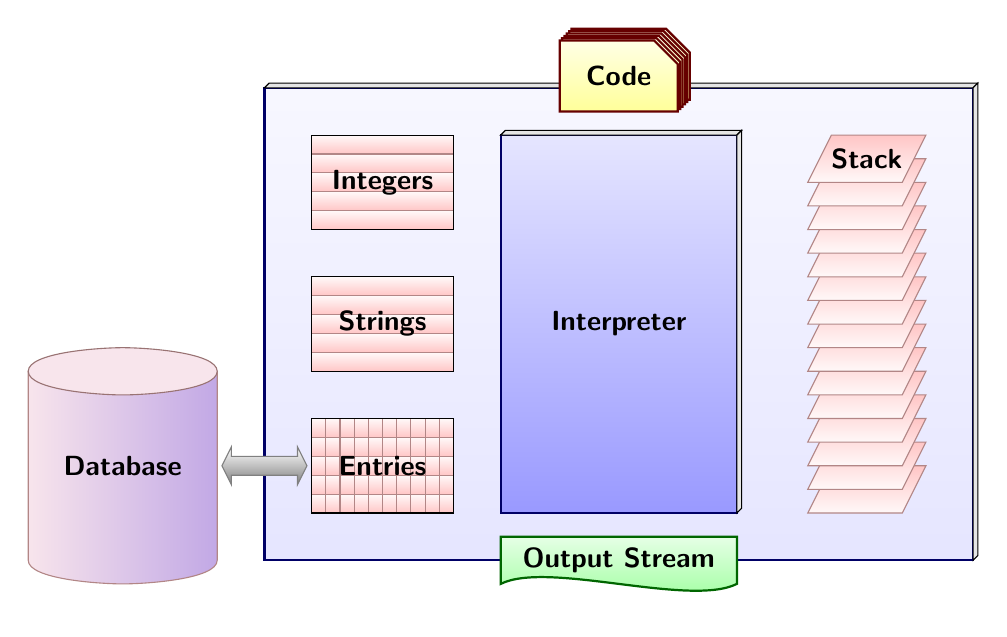
\begin{tikzpicture}[scale=.6]\sf\bfseries
  % --- bottom layer ---
  \shade[top color=white!97!blue,bottom color=white!90!blue,draw=blue!40!black,thick]
  (0,0) rectangle (15,10);
  \draw[fill=gray!20!white] (0,10) -- (.1,10.1) -- (15.1,10.1) -- (15,10) -- cycle;
  \draw[fill=gray!20!white] (15,10) -- (15.1,10.1) -- (15.1,.1) -- (15,0) -- cycle;

  % --- code ---
  \begin{scope}[shift={(6.25,9.5)},scale=.5]
    \begin{scope}[shift={(.5,.5)}]
      \shade[top color=white!90!yellow,bottom color=white!60!yellow,draw=red!40!black,thick]
      (0,0) -- (5,0) -- (5,2) -- (4,3) -- (0,3) -- cycle;
    \end{scope}
    \begin{scope}[shift={(.4,.4)}]
      \shade[top color=white!90!yellow,bottom color=white!60!yellow,draw=red!40!black,thick]
      (0,0) -- (5,0) -- (5,2) -- (4,3) -- (0,3) -- cycle;
    \end{scope}
    \begin{scope}[shift={(.3,.3)}]
      \shade[top color=white!90!yellow,bottom color=white!60!yellow,draw=red!40!black,thick]
      (0,0) -- (5,0) -- (5,2) -- (4,3) -- (0,3) -- cycle;
    \end{scope}
    \begin{scope}[shift={(.2,.2)}]
      \shade[top color=white!90!yellow,bottom color=white!60!yellow,draw=red!40!black,thick]
      (0,0) -- (5,0) -- (5,2) -- (4,3) -- (0,3) -- cycle;
    \end{scope}
    \begin{scope}[shift={(.1,.1)}]
      \shade[top color=white!90!yellow,bottom color=white!60!yellow,draw=red!40!black,thick]
      (0,0) -- (5,0) -- (5,2) -- (4,3) -- (0,3) -- cycle;
    \end{scope}
    \shade[top color=white!90!yellow,bottom color=white!60!yellow,draw=red!40!black,thick]
    (0,0) -- (5,0) -- (5,2) -- (4,3) -- (0,3) -- cycle;
  \end{scope}
  \draw (7.5,10.25) node {Code};

  % --- interpreter ---
  \shade[top color=white!90!blue,bottom color=white!60!blue,draw=blue!40!black,thick]
  (5,1) rectangle (10,9);
  \draw[fill=gray!20!white] (5,9) -- (5.1,9.1) -- (10.1,9.1) -- (10,9) -- cycle;
  \draw[fill=gray!20!white] (10,9) -- (10.1,9.1) -- (10.1,1.1) -- (10,1) -- cycle;
  \draw (7.5,5) node {Interpreter};
  
  \shade[top color=white!90!green,bottom color=white!60!green,draw=green!40!black,thick]
  (5,-.5) .. controls (6,0) and (9,-1) .. (10,-.5) -- (10,.5) -- (5,.5) -- cycle;
  \draw (7.5,0) node {Output Stream};


  % --- stack ---
  \shade[top color=white!10!pink,bottom color=white!90!pink,draw=pink!70!black,shift={(11.5,1)}] (0,0) -- (.5,1) -- (2.5,1) -- (2,0) -- cycle;
  \shade[top color=white!10!pink,bottom color=white!90!pink,draw=pink!70!black,shift={(11.5,1.5)}] (0,0) -- (.5,1) -- (2.5,1) -- (2,0) -- cycle;
  \shade[top color=white!10!pink,bottom color=white!90!pink,draw=pink!70!black,shift={(11.5,2)}] (0,0) -- (.5,1) -- (2.5,1) -- (2,0) -- cycle;
  \shade[top color=white!10!pink,bottom color=white!90!pink,draw=pink!70!black,shift={(11.5,2.5)}] (0,0) -- (.5,1) -- (2.5,1) -- (2,0) -- cycle;
  \shade[top color=white!10!pink,bottom color=white!90!pink,draw=pink!70!black,shift={(11.5,3)}] (0,0) -- (.5,1) -- (2.5,1) -- (2,0) -- cycle;
  \shade[top color=white!10!pink,bottom color=white!90!pink,draw=pink!70!black,shift={(11.5,3.5)}] (0,0) -- (.5,1) -- (2.5,1) -- (2,0) -- cycle;
  \shade[top color=white!10!pink,bottom color=white!90!pink,draw=pink!70!black,shift={(11.5,4)}] (0,0) -- (.5,1) -- (2.5,1) -- (2,0) -- cycle;
  \shade[top color=white!10!pink,bottom color=white!90!pink,draw=pink!70!black,shift={(11.5,4.5)}] (0,0) -- (.5,1) -- (2.5,1) -- (2,0) -- cycle;
  \shade[top color=white!10!pink,bottom color=white!90!pink,draw=pink!70!black,shift={(11.5,5)}] (0,0) -- (.5,1) -- (2.5,1) -- (2,0) -- cycle;
  \shade[top color=white!10!pink,bottom color=white!90!pink,draw=pink!70!black,shift={(11.5,5.5)}] (0,0) -- (.5,1) -- (2.5,1) -- (2,0) -- cycle;
  \shade[top color=white!10!pink,bottom color=white!90!pink,draw=pink!70!black,shift={(11.5,6)}] (0,0) -- (.5,1) -- (2.5,1) -- (2,0) -- cycle;
  \shade[top color=white!10!pink,bottom color=white!90!pink,draw=pink!70!black,shift={(11.5,6.5)}] (0,0) -- (.5,1) -- (2.5,1) -- (2,0) -- cycle;
  \shade[top color=white!10!pink,bottom color=white!90!pink,draw=pink!70!black,shift={(11.5,7)}] (0,0) -- (.5,1) -- (2.5,1) -- (2,0) -- cycle;
  \shade[top color=white!10!pink,bottom color=white!90!pink,draw=pink!70!black,shift={(11.5,7.5)}] (0,0) -- (.5,1) -- (2.5,1) -- (2,0) -- cycle;
  \shade[top color=white!10!pink,bottom color=white!90!pink,draw=pink!70!black,shift={(11.5,8)}] (0,0) -- (.5,1) -- (2.5,1) -- (2,0) -- cycle;
  \draw (12.75,8.5) node {Stack};

  % --- integers ---
  \shade[top color=white!90!pink,bottom color=white!10!pink,draw=pink!70!black]
  (1,7) rectangle (4,7.4);
  \shade[shift={(0,.4)},top color=white!90!pink,bottom color=white!10!pink,draw=pink!70!black]
  (1,7) rectangle (4,7.4);
  \shade[shift={(0,.8)},top color=white!90!pink,bottom color=white!10!pink,draw=pink!70!black]
  (1,7) rectangle (4,7.4);
  \shade[shift={(0,1.2)},top color=white!90!pink,bottom color=white!10!pink,draw=pink!70!black]
  (1,7) rectangle (4,7.4);
  \shade[shift={(0,1.6)},top color=white!90!pink,bottom color=white!10!pink,draw=pink!70!black]
  (1,7) rectangle (4,7.4);
  \draw (1,7) rectangle (4,9);
  \draw (2.5,8) node {Integers};

  % --- strings ---
  \shade[top color=white!90!pink,bottom color=white!10!pink,draw=pink!70!black]
  (1,4) rectangle (4,4.4);
  \shade[shift={(0,.4)},top color=white!90!pink,bottom color=white!10!pink,draw=pink!70!black]
  (1,4) rectangle (4,4.4);
  \shade[shift={(0,.8)},top color=white!90!pink,bottom color=white!10!pink,draw=pink!70!black]
  (1,4) rectangle (4,4.4);
  \shade[shift={(0,1.2)},top color=white!90!pink,bottom color=white!10!pink,draw=pink!70!black]
  (1,4) rectangle (4,4.4);
  \shade[shift={(0,1.6)},top color=white!90!pink,bottom color=white!10!pink,draw=pink!70!black]
  (1,4) rectangle (4,4.4);
  \draw (1,4) rectangle (4,6);
  \draw (2.5,5) node {Strings};

  % --- entries ---
  \shade[top color=white!90!pink,bottom color=white!10!pink,draw=pink!70!black]
  (1,1) rectangle (4,1.4);
  \shade[shift={(0,.4)},top color=white!90!pink,bottom color=white!10!pink,draw=pink!70!black]
  (1,1) rectangle (4,1.4);
  \shade[shift={(0,.8)},top color=white!90!pink,bottom color=white!10!pink,draw=pink!70!black]
  (1,1) rectangle (4,1.4);
  \shade[shift={(0,1.2)},top color=white!90!pink,bottom color=white!10!pink,draw=pink!70!black]
  (1,1) rectangle (4,1.4);
  \shade[shift={(0,1.6)},top color=white!90!pink,bottom color=white!10!pink,draw=pink!70!black]
  (1,1) rectangle (4,1.4);
  \draw[shift={(.3,0)},draw=pink!70!black] (1,1) -- (1,3);
  \draw[shift={(.6,0)},draw=pink!70!black] (1,1) -- (1,3);
  \draw[shift={(.9,0)},draw=pink!70!black] (1,1) -- (1,3);
  \draw[shift={(1.2,0)},draw=pink!70!black] (1,1) -- (1,3);
  \draw[shift={(1.5,0)},draw=pink!70!black] (1,1) -- (1,3);
  \draw[shift={(1.8,0)},draw=pink!70!black] (1,1) -- (1,3);
  \draw[shift={(2.1,0)},draw=pink!70!black] (1,1) -- (1,3);
  \draw[shift={(2.4,0)},draw=pink!70!black] (1,1) -- (1,3);
  \draw[shift={(2.7,0)},draw=pink!70!black] (1,1) -- (1,3);
  \draw (1,1) rectangle (4,3);
  \draw (2.5,2) node {Entries};

  \begin{scope}[shift={(-5,0)}]
    \shade[left color=white!96!blue!70!pink,right color=white!60!blue!60!pink,draw=pink!70!black]
    (0,0)   .. controls (0,-.4) and (1.5,-.5) ..
    (2,-.5)  .. controls (2.5,-.5) and (4,-.4) ..
    (4,0) -- (4,4) -- (0,4) -- cycle;
    \draw[shift={(0,4)},fill=white!96!blue!70!pink,draw=pink!60!black]
    (0,0)   .. controls (0,.4) and (1.5,.5) ..
    (2,.5)  .. controls (2.5,.5) and (4,.4) ..
    (4,0)   .. controls (4,-.4) and (2.5,-.5) ..
    (2,-.5) .. controls (1.5,-.5) and (0,-.4) ..
    (0,0);
  \end{scope}
  \draw (-3,2) node {Database};

%  \draw[shift={(0,-5)}]
%  (-.2,0) -- (0,.4) -- (0,.2) -- (1,.2) -- (1,.4) -- (1.2,0) --
%  (1,-.4) -- (1,-.2) -- (0,-.2) -- (0,-.4) -- cycle;

  \shade[shift={(-.7,2)}, top color=white, bottom color=gray,draw=gray]
  (-.2,0) -- (0,.4) -- (0,.2) -- (1.4,.2) -- (1.4,.4) -- (1.6,0) --
  (1.4,-.4) -- (1.4,-.2) -- (0,-.2) -- (0,-.4) -- cycle;

\end{tikzpicture}
\endgroup
\endinput
%
% Local Variables: 
% mode: latex
% TeX-master: nil
% End: 

  \caption{The BST Programming Model}
  \label{fig:bst-model}
\end{figure}


\subsection{The Database Context}

Whenever a bst program is executed a database is at hand. The porogram
has access to this database.

\INCOMPLETE

\subsection{Global Integers}

\INCOMPLETE

\subsection{Global Strings}

\INCOMPLETE

\subsection{Code}

\INCOMPLETE


\section{Syntax}

\INCOMPLETE

\section{Commands}


\subsection{\texttt{entry}}

\INCOMPLETE

\subsection{\texttt{integers}}

\INCOMPLETE

\begin{lstlisting}{}
  INTEGERS { output.state before.all }
\end{lstlisting}

\subsection{\texttt{strings}}

\INCOMPLETE

\begin{lstlisting}{}
  STRINGS { s t }
\end{lstlisting}

\subsection{\texttt{macro}}

\INCOMPLETE

\begin{lstlisting}{}
  MACRO {jan} {"January"}
\end{lstlisting}

\subsection{\texttt{execute}}

\INCOMPLETE

\begin{lstlisting}{}
  EXECUTE {begin.bib}
\end{lstlisting}

\subsection{\texttt{iterate}}

\INCOMPLETE

\begin{lstlisting}{}
  ITERATE{call.type$}
\end{lstlisting}

\subsection{\texttt{reverse}}

\INCOMPLETE

\begin{lstlisting}{}
  REVERSE{reverse.pass}
\end{lstlisting}

\subsection{\texttt{sort}}

\INCOMPLETE

\begin{lstlisting}{}
  SORT
\end{lstlisting}

\subsection{\texttt{read}}

\INCOMPLETE

\begin{lstlisting}{}
  READ
\end{lstlisting}

\subsection{\texttt{function}}

\INCOMPLETE

\begin{lstlisting}{}
  FUNCTION {sortify}
  { purify$
    "l" change.case$
  }
\end{lstlisting}


\subsection{\texttt{input}}
\IM{x}

\INCOMPLETE

\begin{lstlisting}{}
  INPUT{some/other/bst}
\end{lstlisting}

\section{Instructions}

\subsection{\texttt{>}}

\INCOMPLETE

\subsection{\texttt{<}}

\INCOMPLETE

\subsection{\texttt{=}}

\INCOMPLETE

\subsection{\texttt{+}}

\INCOMPLETE

\subsection{\texttt{-}}

\INCOMPLETE

\subsection{\texttt{*}}

\INCOMPLETE

\subsection{\texttt{:=}}

\INCOMPLETE

\subsection{\texttt{add.period\$}}

\INCOMPLETE

\subsection{\texttt{call.type\$}}

\INCOMPLETE

\subsection{\texttt{change.case\$}}

\INCOMPLETE

\subsection{\texttt{chr.to.int\$}}

\INCOMPLETE

\subsection{\texttt{cite\$}}

\begin{lstlisting}{}
  cite$
\end{lstlisting}

\INCOMPLETE

\subsection{\texttt{duplicate\$}}

\INCOMPLETE

\subsection{\texttt{empty\$}}

\INCOMPLETE

\subsection{\texttt{format.name\$}}

\INCOMPLETE

\subsection{\texttt{if\$}}

\INCOMPLETE

\subsection{\texttt{int.to.chr\$}}

\INCOMPLETE

\subsection{\texttt{int.to.str\$}}

\INCOMPLETE

\subsection{\texttt{missing\$}}

\INCOMPLETE

\subsection{\texttt{newline\$}}

This instruction writes a newline character to the output stream.

\begin{lstlisting}{}
  newline$
\end{lstlisting}

\subsection{\texttt{num.names\$}}

\INCOMPLETE

\subsection{\texttt{pop\$}}

\INCOMPLETE

\subsection{\texttt{preamble\$}}

\INCOMPLETE

\subsection{\texttt{purify\$}}

\INCOMPLETE

\subsection{\texttt{quote\$}}

\INCOMPLETE

\subsection{\texttt{skip\$}}

This instruction does simply nothing. In other languages this might be
called a noop. This is useful for places where instructions are
mandatory but nothing should be done.

\subsection{\texttt{stack\$}}

\INCOMPLETE

\subsection{\texttt{substring\$}}

\INCOMPLETE

\subsection{\texttt{swap\$}}

This instruction takes the two topmost elements from the stack and
exchanges their order on the stack. This means that the topmost
element becomes the second one and the second element becomes the
topmost one. The elements can be of any type.

If there are less than two elements on the stack then an error is
raised.

\subsection{\texttt{text.length\$}}

\INCOMPLETE

\subsection{\texttt{text.prefix\$}}

\INCOMPLETE

\subsection{\texttt{top\$}}

\INCOMPLETE

\subsection{\texttt{type\$}}

\INCOMPLETE

\subsection{\texttt{warning\$}}

This instruction pops a string from the stack and prints it as a
warning to the log stream.

\subsection{\texttt{while\$}}

\INCOMPLETE

\subsection{\texttt{width\$}}

This instruction pops a string from the stack and tries to compute the
width of the string when tyoeset. For this purpose the width of the
characters in the font cmr10 are used.

\subsection{\texttt{write\$}}

This instruction pops a string from the stack and prints it as a
message to the output stream.


\endinput
%
% Local Variables: 
% mode: latex
% TeX-master: "exbib-users"
% End: 

\ifdraft\else%%*****************************************************************************
%% Copyright (c) 2008-2010 Gerd Neugebauer
%%
%% Permission is granted to copy, distribute and/or modify this document
%% under the terms of the GNU Free Documentation License, Version 1.2
%% or any later version published by the Free Software Foundation;
%% with no Invariant Sections, no Front-Cover Texts, and no Back-Cover Texts.
%%
%%*****************************************************************************
%% $Id$
%%*****************************************************************************
%% Author: Gerd Neugebauer
%%-----------------------------------------------------------------------------

\section{More Style Languages}

The Bean Scripting Framework (\url{http://bsf.apache.org}) provides a
convenient way to integrate additional scripting languages into
\ExBib. Several languages have been prepared this way. Thus they can
be used instead of the BST language.

%%*****************************************************************************
%% Copyright (c) 2008-2010 Gerd Neugebauer
%%
%% Permission is granted to copy, distribute and/or modify this document
%% under the terms of the GNU Free Documentation License, Version 1.2
%% or any later version published by the Free Software Foundation;
%% with no Invariant Sections, no Front-Cover Texts, and no Back-Cover Texts.
%%
%%*****************************************************************************
%% $Id: bsf.tex 8314 2010-11-21 19:06:53Z gene $
%%*****************************************************************************
%% Author: Gerd Neugebauer
%%-----------------------------------------------------------------------------

\newenvironment{methods}{\begin{description}\def\method##1{\item[##1]\ \\}%
}{\end{description}}
\definecolor{UMLclassColor}{rgb}{1,1,.72}
\definecolor{UMLclassLineColor}{rgb}{.8,.25,.25}
\newbox\UMLbox
\newenvironment{UMLclass}[1]{\scriptsize
  \arrayrulewidth=.75pt
  \setbox\UMLbox=\hbox\bgroup\tt
    \begin{tabular}{l}
      \textbf{#1}\\\hline\hline
}{%
      \\
    \end{tabular}\egroup
    \begin{center}
      \fboxrule 1pt \fboxsep=0pt
      \fcolorbox{UMLclassLineColor}{UMLclassColor}{\usebox\UMLbox}%
    \end{center}%
}


\section{Groovy as Style Language}

An experimental feature of \ExBib{} is the replanceemnt of the BST
language by some other language for writing styles. Here the Bean
Scripting Framework (BSF) is used as adapter for other languages. Any
language made available this way can be plugged in with minor effort
as style language.

As an example the language Groovy has been made available this way.


\subsection{Invoking the Groovy-enhanced \ExBib}

The property \Property{exbib.processor} determines which processor is
used. The value of this property must be set to th value \verb|groovy|
to activate the Groovy entension language. In the simplest case this
is done on the command line as shown in the following example:

\begin{lstlisting}[language=sh]
# exbib -Dexbib.processor=groovy myDocument.aux
\end{lstlisting}

If you want to activate this property for any invocation of \ExBib\ in
this directory then you can alternatively create a file named
\File{.exbib} in the current directory. This file should contain the
following line:

\begin{lstlisting}
exbib.processor=groovy
\end{lstlisting}

Then the usual invocation uses the Groovy extension instead of bst
style files:

\begin{lstlisting}[language=sh]
# exbib myDocument.aux
\end{lstlisting}

See also section \ref{sec:dot.files} for details.


\subsection{Specifying a Groovy Style}

A Groovy style file can be specified in the same way a bst style file
is given. In \LaTeX\ the command \Macro{bibliographystlye} writes the
name of the style file is written to the aux file. The name of the
style file is given without any extension -- like \verb|.gy| or
\verb|.groovy| for Groovy files.


\subsection{Accessing the Database in a Groovy Style}

The databases specified in the aux file are automaticaly read at
startup. The code contained in the Groovy style is executed after the
database has been read in. The database can be accessed via the global
variable \Var{bibDB}. This variable contains an object which
implements the interface \texttt{org.extex.exbib.core.db.DB}. The full
power of this Java interface is described in the Javadoc.


\subsection{The Output}

The global variable \Var{bibWriter} contains an instance of a class
implementing the interface \texttt{org.extex.exbib.core.io.Writer}.
This writer can be used to write to the output file.

It has a method \Method{print} to print some strings:

\begin{lstlisting}[language=Java]
  bibWriter.print("{\em ", series, "\/}" )
\end{lstlisting}

It has a method \Method{println} to print some strings followed by a
newline character:

\begin{lstlisting}[language=Java]
  bibWriter.println("\newcommand{\etalchar}[1]{$^{#1}$}" )
\end{lstlisting}


\subsection{The Processor Context}\label{sec:groovy.processor}

The processor context is defined in the interface \texttt{Processor}.
The processor can be accesed through the global variable
\Var{bibProcessor}. This gives access to additional features like the
log file.

\begin{UMLclass}{Processor}
  String getCite(String key)\\
  DB getDB()\\
  List<String> getEntries()\\
  Logger getLogger()\\
  String getMacro(String name)\\
  List<String> getMacroNames()\\
  long getNumberOfWarnings()\\
  Writer getOutWriter()\\
  boolean isKnown(String type)\\
  void warning(String message)
\end{UMLclass}

\begin{methods}

  \method{String getCite(String key)}\MethodIndex{getCite}%
    Get the original cite key for a given key. I.e. the casing might be
    different.

  \method{DB getDB()}\MethodIndex{getDB}%
    Getter for the database. The same database is accessible via the
    global variable \Var{bibDB} as well for convenience.

  \method{List<String> getEntries()}\MethodIndex{getEntries}%
    Getter for the entries.

  \method{Logger getLogger()}\MethodIndex{getLogger}%
    Getter for the logger.

  \method{String getMacro(String name)}\MethodIndex{getMacro}%
    Getter for a certain macro. If the requested macro is not defined
    \texttt{null} is returned.

  \method{List<String> getMacroNames()}\MethodIndex{getMacroNames}%
    Getter for the list of all defined macro names.

  \method{long getNumberOfWarnings()}\MethodIndex{getNumberOfWarnings}%
    Getter for the number of warnings issued.

  \method{Writer getOutWriter()}\MethodIndex{getOutWriter}%
    Getter for the output writer. This is the same value as the one
    provided in the variable \Var{bibWriter}.

  \method{boolean isKnown(String type)}\MethodIndex{isKnown}%
    Check if the entry type is known.

  \method{void warning(String message)}\MethodIndex{warning}%
    This method can be used to issue a warning message.

\end{methods}


\subsection{Methods of a DB}\label{sec:groovy.db}

The important methods of the DB provide reading access to the stored
information. The DB is defined in the interface \texttt{org.extex.exbib.core.db.DB}.
The important methods are described below.

\begin{UMLclass}{DB}
  Entry getEntry(String key)\\
  String getExpandedMacro(String key)\\
  Value getMacro(String name)\\
  List<String> getMacroNames()\\
  int getMinCrossrefs()\\
  Value getPreamble()\\
  String getPreambleExpanded()\\
  void setMinCrossrefs(int minCrossref)\\
  void sort() throws ConfigurationException
\end{UMLclass}

\begin{methods}
  \method{Entry getEntry(String key)}\MethodIndex{getEntry}%
    Get a single entry stored under the given reference key. The key
    is normalized before the entry is sought, i.e. the search is case
    insensitive.
    
    If no record is stored under the given key then <code>null</code>
    is returned.

  \method{String getExpandedMacro(String key)}\MethodIndex{getExpandedMacro} %
    Compute the expanded representation of a macro. The expansion is
    performed by recursively replacing macro names by the definitions
    and concatenating the resulting list of values.
    
    For any macro which is not defined during the expansion the empty
    string is used instead.
    
    If the named macro the expansion is started with does not exist
    then \texttt{null} is returned.

  \method{Value getMacro(String name)}\MethodIndex{getMacro}%
    Retrieve the definition of a macro.

  \method{List<String> getMacroNames()}\MethodIndex{getMacroNames}%
    Retrieve the list of macro names.

  \method{int getMinCrossrefs()}\MethodIndex{getMinCrossrefs}%
    Getter for minCrossrefs.
    
    The parameter minCrossrefs determines when an entry which is
    referenced by several entries should be collated into the
    referencing entries. For example this can be the case for articles
    in a collection. Here the collection is shown as separate entry
    only if at least minCrossref entries in the result reference it.

  \method{Value getPreamble()}\MethodIndex{getPreamble}%
    Getter for the preamble.

  \method{String getPreambleExpanded()}\MethodIndex{getPreambleExpanded}%
    Getter for the preamble with all constituents expanded and combined into
    one string.

  \method{void setMinCrossrefs(int minCrossref)}\MethodIndex{setMinCrossrefs}%
    Setter for minCrossrefs.

  \method{void sort() throws ConfigurationException}\MethodIndex{sort}%
    Sort the entries according to the configured sorter.
    Initially the entries are in the order in which they are read in.

\end{methods}

\subsection{Methods of an Entry}\label{sec:groovy.entry}

The entry is defined in the class
\texttt{org.extex.exbib.core.db.Entry}. The entry describes an entry
in the database, i.e. a dabase record. It has several properties and
some fixed values.
The important methods are described below.

\begin{UMLclass}{Entry}
  Value get(String key, DB db) throws ExBibException\\
  String getExpanded(String key, DB db) throws ExBibException\\
  String getKey()\\
  List<String> getKeys()\\
  ValueItem getLocal(String key)\\
  int getLocalInt(String key)\\
  String getLocalString(String key)\\
  Locator getLocator()\\
  String getSortKey()\\
  String getType()\\
  Iterator<String> iterator()\\
  void set(String key, String value)\\
  void set(String key, Value value)\\
  setKey(String key)\\
  void setLocal(String key, int value)\\
  void setLocal(String key, String value)\\
  void setLocal(String key, ValueItem value)\\
  void setSortKey(String sortKey)\\
  void setType(String t)\\
  String toString()
\end{UMLclass}

\begin{methods}
  \method{Value get(String key, DB db) throws ExBibException}\MethodIndex{get}%
    Getter for the Value stored under a given key in the Entry. If the
    value is not found locally and the field crossref is present then
    the value is requested from the entry stored under the crossref key
    in the database.

  \method{String getExpanded(String key, DB db) throws ExBibException}\MethodIndex{getExpanded}%
    This method searches for a normal value and concatenates all
    expanded constituents. Macros are looked up in the database given and
    their values are inserted.

  \method{String getKey()}\MethodIndex{getKey}%
    Getter for the reference key for this Entry.

  \method{List<String> getKeys()}\MethodIndex{getKeys}%
    Getter for the list of keys for "normal" values. Note that those keys may
    lead to \texttt{null} values..

  \method{ValueItem getLocal(String key)}\MethodIndex{getLocal}%
    Getter for a local value. The local values are stored independently from
    the normal values. This means that they have a name-space of their own.

  \method{int getLocalInt(String key)}\MethodIndex{getLocalInt}%
    Getter for a local value. The local values are stored independently from
    the normal values. This means that they have a name-space of their own.

  \method{String getLocalString(String key)}\MethodIndex{getLocalString}%
    Getter for a local value. The local values are stored independently from
    the normal values. This means that they have a name-space of their own.

  \method{Locator getLocator()}\MethodIndex{geLocatort}%
    Getter for the locator for this Entry. The locator allows you to
    determine where this Entry is coming from.

  \method{String getSortKey()}\MethodIndex{getSortKey}%
    Getter for the sort key of this Entry. The sort key is stored as local
    value under the key \texttt{sort.key\$}.

  \method{String getType()}\MethodIndex{getType}%
    Getter for the type of this Entry.

  \method{Iterator<String> iterator()}\MethodIndex{iterator}%
    Getter for an iterator over all keys of normal values.

  \method{void set(String key, String value)}\MethodIndex{set}%
    Setter for the Value stored under a given key in the Entry. The String
    valued parameter is wrapped into a  Value before it is stored.

  \method{void set(String key, Value value)}\MethodIndex{set}%
    Setter for the Value stored under a given key in the Entry. An already
    existing value is overwritten silently.

  \method{setKey(String key)}\MethodIndex{setKey}%
    Setter for the reference key for this Entry.

  \method{void setLocal(String key, int value)}\MethodIndex{setLocal}%
     Setter for a local value. The local values are stored independently from
     the normal values. This means that they have a namespace of their own.

    This method wraps its int argument into a VNumber before it is stored.

  \method{void setLocal(String key, String value)}\MethodIndex{setLocal}%
     Setter for a local value. The local values are stored independently from
     the normal values. This means that they have a namespace of their own.

     This method wraps its int argument into a VString before it is stored.

  \method{void setLocal(String key, ValueItem value)}\MethodIndex{setLocal}%
    Setter for a local value. The local values are stored independently
    from the normal values. This means that they have a name-space of
    their own.

  \method{void setSortKey(String sortKey)}\MethodIndex{setSortKey}%
    Setter for the sort key of this Entry. The sort key is stored as
    local value under the key \texttt{sort.key\$}.

  \method{void setType(String t)}\MethodIndex{setType}%
    Setter for the type of this Entry.

  \method{String toString()}%
    Return a string representation of the object. Ths is for debugging
    and for reading it back in.
\end{methods}

\subsection{Methods of a Value}\label{sec:groovy.value}

The values are used as the right hand side of a entry item. It is a list of
\texttt{ValueItem}s.

\begin{UMLclass}{Value}
  void add(Value item)\\
  void add(ValueItem item)\\
  String expand(DB db)\\
  boolean isEmpty()\\
  Iterator<ValueItem> iterator()  
\end{UMLclass}

\begin{methods}
  \method{void add(Value item)}\MethodIndex{add}%
    Add all value items contained in a value to the current value.

  \method{void add(ValueItem item)}\MethodIndex{add}%
    Add a new value item to the end of the value.

  \method{String expand(DB db)}\MethodIndex{expand}%
    Expand the whole value into a single String. All macros are replaced by
    their values and delimiting braces or quotes are omitted.

  \method{boolean isEmpty()}\MethodIndex{isEmpty}%
    Tests whether the value is empty.

  \method{Iterator<ValueItem> iterator()}\MethodIndex{iterator}%
    Getter for an Iterator for all elements.
\end{methods}


\subsection{Methods of a ValueItem}\label{sec:groovy.valueitem}

A ValueItem is an object stored as a part of a \texttt{Value}. It is an
interface for which the implementations \texttt{VBlock}, \texttt{VMacro},
\texttt{VNumber}, and \texttt{VString} are present. 

\begin{UMLclass}{ValueItem}
  void expand(StringBuilder sb, DB db)\\
  String getContent()\\
  void setContent(String value)
\end{UMLclass}

\begin{methods}

  \method{void expand(StringBuilder sb, DB db)}\MethodIndex{expand}%
    This method expands the ValueItem and appends the expansion to the given
    StringBuilder. Macros are looked up in the database given and their
    values are inserted.

  \method{String getContent()}\MethodIndex{getContent}%
    The getter for the content.

  \method{void setContent(String value)}\MethodIndex{setContent}%
    Setter for the content.

\end{methods}


\subsection{Methods of a Locator}\label{sec:groovy.locator}

The locator is a means to determine where something is coming from.

\begin{UMLclass}{Locator}
  int getLineNumber()\\
  int getLinePointer()\\
  String getResourceName()
\end{UMLclass}

\begin{methods}

  \method{int getLineNumber()}\MethodIndex{getLineNumber}%
    Getter for the line number.

  \method{int getLinePointer()}\MethodIndex{getLinePointer}%
    Getter for the position in the line.

  \method{String getResourceName()}\MethodIndex{getResourceName}%
    Getter for the resource name. The resource can be a file or the content of
    a URL or a member of an archive or something else. It is a general concept
    whch can be used as needed.

\end{methods}

\subsection{Methods of a List}\label{sec:groovy.list}

Lists are ordered containers of typed elements. This menay they
contain for instance Strings or Entrries. Since the lists are just
used as return values in the interface to \ExBib\ only the reading
methods are described below.

\begin{UMLclass}{List<ElementType>}
  boolean isEmpty()\\
  int size()\\
  <\textit{ElementType}> get(int index)
\end{UMLclass}

\begin{methods}
  \method{boolean isEmpty()}\MethodIndex{isEmpty}%
    Getter for an indicator whethger or not the list is empty, i.e.
    does not contain any element.
  \method{int size()}\MethodIndex{size}%
    Getter for the number of elements in the list.
  \method{\textit{ElementType} get(int index)}\MethodIndex{get}%
    Getter for a certain element in the list. The element is addressed
    via an index. The index is 0-based. Thus the index needs to be in
    the range $[0,size()-1]$. If an invalid index is used then an
    Exception is thrown.
\end{methods}

\subsection{Methods of a Logger}\label{sec:groovy.logger}

The logger is used to record log messages. The logger talkes care to
put the messages to the appripriate place, i.e. it takes care to write
them to a log file or present them on the console.

The log messages are categorized with certain log levels. Based on
these log levels the logger can be configured to suppress messages
below a certain level for an output channel.

\begin{UMLclass}{Logger}
  void fine()\\
  void finer()\\
  void finest()\\
  void info()\\
  void warning()\\
  void severe()
\end{UMLclass}

\begin{methods}
  \method{void fine()}\MethodIndex{fine}%
    Write a log message with the log level ``fine''. Usually any
    message of this kind and below is suppressed.
  \method{void finer()}\MethodIndex{finer}%
    Write a log message with the log level ``finer''.
  \method{void finest()}\MethodIndex{finest}%
    Write a log message with the log level ``finest''. This is the
    lowest level.
  \method{void info()}\MethodIndex{info}%
    Write a log message with the log level ``info''.
  \method{void warning()}\MethodIndex{warning}%
    Write a log message with the log level ``waring''.
  \method{void severe()}\MethodIndex{severe}%
    Write a log message with the log level ``severe''. This is the
    highest level.
\end{methods}

\subsection{Methods of a Writer}\label{sec:groovy.writer}

A writer provides means to write something to a destination. Thus the
most important method is described below:

\begin{methods}
  \method{void write(String str)}\MethodIndex{write}%
    Write the string to the output destination.
\end{methods}


\subsection{Accessing \BibTeX\ Functions}

Sometimes it is desirable to have access to the original or enhanced
function of the \BibTeX\ style language. There are two ways to access
them. The complex functions -- which are likely to be needed this way
-- are provided as static methods of implementing classes. All
functions can be accesed via implementing function objects.

The implementation classes described below can be found in a Java
package This packege is \texttt{org.extex.exbib.core.bst.code.impl}.
It must be used for the imports of the classes or for direct refernce.

\begin{methods}

  \method{String ChangeCase.changeCase(String type, String string)}\MethodIndex{changeCase}%
  Apply the function \texttt{change.case\$}\fctIndex{change.case\$}.

  \method{String FormatName.formatName(String names, int index, String format)}\MethodIndex{formatName}%
  Apply the function \texttt{format.name\$}\fctIndex{format.name\$}.

  \method{String NumNames.numNames(String names)}\MethodIndex{numNames}%
  Apply the function \texttt{num.names\$}\fctIndex{num.names\$}.

  \method{String Purify.purify(String string)}\MethodIndex{purify}%
  Apply the function \texttt{purify\$}\fctIndex{purify\$}.

  \method{String Substring.substring(String string, int startIndex, int endIndex)}\MethodIndex{substring}%
  Apply the function \texttt{substring\$}\fctIndex{substring\$}.

  \method{int TextLength.textLength(String string)}\MethodIndex{textLength}%
  Apply the function \texttt{text.length\$}\fctIndex{text.length\$}.

  \method{int Width.width(String string)}\MethodIndex{width}%
  Apply the function \texttt{width\$}\fctIndex{width\$}.

\end{methods}
\endinput%%%%%%%%%%%%%%%%%%%%%%%%%%%%%%%%%%%%%%%%%%%%%%%%%%%%%%%%%%%%%%%%%%%%%%
%
% Local Variables: 
% mode: latex 
% TeX-master: "../exbib-manual"
% End:


\endinput%%%%%%%%%%%%%%%%%%%%%%%%%%%%%%%%%%%%%%%%%%%%%%%%%%%%%%%%%%%%%%%%%%%%%%
%
% Local Variables: 
% mode: latex 
% TeX-master: "../exbib-manual"
% End:

\fi
%%*****************************************************************************
%% $Id: tex-aux.tex,v 0.00 2008/05/02 01:07:48 gene Exp $
%%*****************************************************************************
%% Author: Gerd Neugebauer
%%-----------------------------------------------------------------------------

\chapter{Behind the Scenes}

\section{The \texttt{aux} File}


\IM{08x1} The selection of databases and entries in \ExBib\ is mainly
controlled by the \texttt{aux} file. The aux file is usually prouced
by \LaTeX\index{LaTeX@\LaTeX} and read by \ExBib. Since the aux file
is also used to communicate between successive runs of \LaTeX\ it can
contain information not relevant for \ExBib. This irrelevant
information is ignored.

Whenever the \texttt{aux} file is read the relevant information is
found by a strict pattern matching. The macros described below will be
recognized only if they are on a line by their own. Any characters
preceeding or following them on the same line will lead to the
skipping when the \texttt{aux} file is read.

\subsection{The Declaration of Databases}
\INCOMPLETE

\begin{lstlisting}{}
  \bibdata{the/bibliography}
\end{lstlisting}

\subsection{The Declaration of Citations}
\INCOMPLETE

\begin{lstlisting}{}
  \citation{a.label,another.label}
\end{lstlisting}

\subsection{The Declaration of the Style}
\INCOMPLETE

\begin{lstlisting}{}
  \bibstyle{the/style}
\end{lstlisting}

\INCOMPLETE

\subsection{The Declaration of Includes}
\begin{lstlisting}{}
  \@include{the/included/file}
\end{lstlisting}

\INCOMPLETE

\endinput
%
% Local Variables: 
% mode: latex
% TeX-master: "../exbib-manual"
% End: 

%%*****************************************************************************
%% Copyright (c) 2008 Gerd Neugebauer
%%
%% Permission is granted to copy, distribute and/or modify this document
%% under the terms of the GNU Free Documentation License, Version 1.2
%% or any later version published by the Free Software Foundation;
%% with no Invariant Sections, no Front-Cover Texts, and no Back-Cover Texts.
%%
%%*****************************************************************************
%% $Id:configuration.tex 7067 2008-05-18 11:06:56Z gene $
%%*****************************************************************************
%% Author: Gerd Neugebauer
%%-----------------------------------------------------------------------------


\section{Configuring \ExBib}

\subsection{Locating the Configuration}

If you are looking for the configurations in the distribution or want
to provide a configuration of your own you need to know how a
configuraion is found. \ExBib\ has a general mechanism for finding
resources. Unfortunately this mechanism can not be used for the
configuration since it is defined in the configuration itself. Thus
the location of a configuration uses a simpler search.

There are two places where \ExBib\ looks for a configuration. Those
are mainly located in the \ExBib\ installation directory (cf.
section~\ref{sec:inst.dir}).
\begin{itemize}
\item The current directory may contain a configuration with the
  proper name and path.
\item The directory \File{config} in the \ExBib\ installation
  directory contains an unpacked directory tree. Any configuration in
  this directory tree with a proper name and path is considered.
\item The directory \File{lib} in the \ExBib\ installation directory
  contains jar archives. Any configuration in a jar archive with a
  proper name and path is considered.
\end{itemize}

The top level configuration file is located with the path
\texttt{exbib}. The prefix \texttt{config/} is tried first; then the
name withpout prefix. The configuration is used with the additional
extension \texttt{.xml} and as given. Thus the configuration
\texttt{cfg} passed in as property or via the command line is sought
with the following full names:
\begin{verbatim}
  config/exbib/cfg.xml
  config/exbib/cfg
  exbib/cfg.xml
  exbib/cfg
\end{verbatim}


\subsection{Extracting a Configuration from an Archive}

To get started you may want to examine the configurations in a jar
archive. This can be accomplished with the program \Prog{jar} whoich
is part of the installed Java. We assume that the program can be found
on your search path for executables.

First you can list the files as follows:
\begin{lstlisting}[language=sh]
  # jar -tvf exbib.jar
\end{lstlisting}

Then you can extract the files you want from the archive
\begin{lstlisting}[language=sh]
  # jar -xvf exbib.jar config/exbib/exbib.xml
\end{lstlisting}

Note that a directory tree is created containing the extracted files.


\subsection{The Configuration Format}

The configuration files are XML files. The default configuration file
(\File{exbib.xml}) contains the following definitions:

\begin{lstlisting}[language=XML]
<exbib fallback="bbl">
  <Resource src="path/exbibFinder"/>
  <Processor base="exbib/processor/" default="exbib"/>
  <BblWriter class="org.extex.exbib.core.io.bblio.BblWriter">
    <linelength>79</linelength>
    <indent>  </indent>
  </BblWriter>
  <DB class="org.extex.exbib.core.db.impl.DBImpl">
    <minCrossrefs>2</minCrossrefs>
  </DB>
  <Sorter base="exbib/sorter/" default="locale"/>
  <AuxReader class="org.extex.exbib.core.io.auxio.AuxReaderImpl"/>
  <BibReader class="org.extex.exbib.core.io.bibio.BibReaderImpl"/>
  <BibPrinter base="exbib/printer/" default="bib"/>
</exbib>
\end{lstlisting}


\INCOMPLETE


\endinput
%
% Local Variables: 
% mode: latex
% TeX-master: "../exbib-manual"
% End: 

%%*****************************************************************************
%% $Id:finder.tex 7067 2008-05-18 11:06:56Z gene $
%%*****************************************************************************
%% Author: Gerd Neugebauer
%%-----------------------------------------------------------------------------

\def\LogArg#1{$\langle${\itshape #1}$\rangle$}

\section{Finding Files and Resources}

All inputs needed are called resources. In the simplest case those
resources are plain files. Whenever a resource is needed a search for
it takes place. We will see how the search works and how it can be
influenced.


\subsection{The Configuration File}

\ExBib\ inherits its resource search from \ExTeX\index{ExTeX@\ExTeX}.
This resource search is rather flexible and highly configurable. With
this respect it follows the path defined by kpathsea\index{kpathsea}.

The search for a resource can be configured in a configuration file.
This configuration files utilizes resource finders which have a
configuration section each.

\INCOMPLETE


\subsection{Tracing the Search}

The tracing can be activated with the trace attributes for some
sections or globally for the whole search at runtime. As a consequence
the log file should contain messages describing the search -- where it
looked and what it found.


\subsection{File Search in the Directory Tree}

The simplest search strategy is to look into a list of directories and
maybe try a list of extensions until a suitable file is found. This
strategy is implemented in the class
\texttt{org.extex.resource.FileFinder}.

\subsubsection*{Example}

\begin{lstlisting}[language=XML]
  <Finder class="org.extex.resource.FileFinder"
          default="default">
    <default>
      <path>.</path>
      <path property="extex.texinputs"/>
      <path property="texinputs"/>
      <path env="EXTEX_TEXINPUTS"/>
      <path env="TEXINPUTS"/>
      <extension>.{type}</extension>
      <extension/>
    </default>
  </Finder>
\end{lstlisting}

\subsubsection*{Attributes}
\begin{description}
\item[class] The attribute \texttt{class} has the value
  \texttt{org.extex.resource.FileFinder} for the search in
  archives. It is mandatory.
\item[default] The attribute \texttt{default} names the type shich
  should be used if no special section for the type at hand is
  present. This attribute is mandatory.
\item[trace] The attribute \texttt{trace} can be used to turn on the
  tracing from within the configuration. It takes a boolean value as
  argument (\texttt{true} or \texttt{false}). The tracing can be
  overwritten at runtime. This attribute is optional. The default
  value is \texttt{false}.
\end{description}

\subsubsection*{Nested Elements}

The nested elements are used to select the parameters for the type of
the resource in question. The nested element with the same name as the
type is used. If no such nested element is found then the value of the
\texttt{default} attribute is used to read this nested element
instead. 

The nested element found must contain nested elements with the name
\texttt{extension}. The values of those nested \texttt{extension}
elements are appended to the resource name when it is sought.

The nested element found must contain a nested element named
\texttt{path}. It is treated as follows:
\begin{itemize}
\item If the attribute \texttt{property} is given then the body is
  ignored and the directory read from the named property.
\item If the attribute \texttt{env} is given then the body is ignored
  and the directory read from the named environment variable.
\item Otherwise the body is used as directory.
\end{itemize}

The file is constructed from the path, the resource name and the
extension. The string \verb|{.type}| in the constructed resource name
is replaced by the currently sought resource. This value can occur in
the extension or the path. The first readable resource wins.

\subsubsection*{Tracing Output}

The following messages might be written to the log:

{\small
\begin{itemize}
\item{\tt FileFinder: Searching \LogArg{name} [\LogArg{type}]}
\item{\tt FileFinder: Trying \LogArg{full name}}
\item{\tt FileFinder: Found \LogArg{full name}}
\item{\tt FileFinder: Not found \LogArg{name}}
\item{\tt FileFinder: Failed for \LogArg{name}}
\item{\tt FileFinder: Property \LogArg{property name} is undefined.}
\item{\tt FileFinder: Environment variable \LogArg{env} is undefined.}
\item{\tt FileFinder: Configuration for `\LogArg{type}' not found;
    Using default `\LogArg{element name}'}
\end{itemize}}

Note that the messages are subject to internationalization. Thus a
translated version can appear for other user languages than English.


\subsection{Searching in texmf Trees}

The search in texmf utilizes the index file \File{ls-R}. If this file
is not found then the directory is ignored. The index file \File{ls-R}
is read in and used to find the resources.

\subsubsection*{Example}

\begin{lstlisting}[language=XML]
  <Finder class="org.extex.resource.LsrFinder"
          trace="false"
          capacity="88888"
          default="default">
    <path property="extex.texinputs"/>
    <path property="texinputs"/>
    <path env="EXTEX_TEXINPUTS"/>
    <path env="TEXINPUTS"/>

    <default>
      <extension>.{type}</extension>
      <extension/>
    </default>
  </Finder>
\end{lstlisting}

\subsubsection*{Attributes}
\begin{description}
\item[class] The attribute \texttt{class} has the value
  \texttt{org.extex.resource.LsrFinder} for the search in archives. It
  is mandatory.
\item[default] The attribute \texttt{default} names the type which
  should be used if no special section for the type at hand is
  present. This attribute is mandatory.
\item[capacity] The attribute \texttt{capacity} gives an initial
  capacity for the size of the hash used to store the index entries
  from the \File{ls-R} files. Its fallback is rather small and the
  performance can be influenced positively by using this attribute
  with a proper value.
\item[trace] The attribute \texttt{trace} can be used to turn on the
  tracing from within the configuration. It takes a boolean value as
  argument (\texttt{true} or \texttt{false}). The tracing can be
  overwritten at runtime. This attribute is optional. The default
  value is \texttt{false}.
\end{description}

\subsubsection*{Nested Elements}

The nested elements are used to select the parameters for the type of
the resource in question. The nested element with the same name as the
type is used. If no such nested element is found then the value of the
\texttt{default} attribute is used to read this nested element
instead. 

The nested element found may contain nested elements with the name
\texttt{extension}. The values of those nested \texttt{extension}
elements are appended to the resource name when it is sought in the
index. The first readable resource wins.

The string \verb|{.type}| in the constructed resource name is replaced
by the currently sought resource. This value can occur in the
extension.

One nested element is treated special:

\begin{description}
\item[path] The nested element \texttt{path} specified where to look
  for the index file \File{ls-R}. There are several cases in which
  this nested element can be used:
  \begin{itemize}
  \item If the attribute \texttt{property} is given then the body is
    ignored and the directory read from the named property.
  \item If the attribute \texttt{env} is given then the body is
    ignored and the directory read from the named environment
    variable.
  \item Otherwise the body is used as directory to search the index
    file \File{ls-R}.
  \end{itemize}
\end{description}

\subsubsection*{Tracing Output}

The following messages might be written to the log:

{\small
\begin{itemize}
\item{\tt LsrFinder: Searching \LogArg{name} [\LogArg{type}]}
\item{\tt LsrFinder: Trying \LogArg{full name}}
\item{\tt LsrFinder: Found \LogArg{full name}}
\item{\tt LsrFinder: Ignoring unreadable file \LogArg{full name}}
\item{\tt LsrFinder: Database \LogArg{index} is not readable}
\item{\tt LsrFinder: Failed for \LogArg{name}}
\item{\tt LsrFinder: Loaded database file `\LogArg{index}' in \LogArg{time} ms, size=\LogArg{size}}
\item{\tt LsrFinder: Property \LogArg{property name} is undefined.}
\item{\tt FileFinder: Environment variable \LogArg{env} is undefined.}
\item{\tt LsrFinder: Configuration for `\LogArg{type}' not found;
    Using default `\LogArg{element name}'}
\item{\tt LsrFinder: Default configuration not found}
\item{\tt LsrFinder: Type `\LogArg{type}' skipped}
\end{itemize}}

Note that the messages are subject to internationalization. Thus a
translated version can appear for other user languages than English.


\subsection{Recursively Searching in Directory Trees}

Resources can be sought somewhere in a directory. This means in the
directory or recursivle in one of its sub-directories. This method
really traverses the directory tree. This is not advisable since it
can be rather slow.

\subsubsection*{Example}

\begin{lstlisting}[language=XML]
  <Finder class="org.extex.resource.FileFinderRPath"
          trace="false"
          default="default">>
    <path property="extex.texinputs"/>
    <path property="texinputs"/>

    <default>
      <extension>.{type}</extension>
      <extension/>
    </default>
  </Finder>
\end{lstlisting}


\subsubsection*{Attributes}
\begin{description}
\item[class] The attribute \texttt{class} has the value
  \texttt{org.extex.resource.FileFinderRPath} for the search in
  archives. It is mandatory.
\item[default] The attribute \texttt{default} names the type shich
  should be used if no special section for the type at hand is
  present. This attribute is mandatory.
\item[trace] The attribute \texttt{trace} can be used to turn on the
  tracing from within the configuration. It takes a boolean value as
  argument (\texttt{true} or \texttt{false}). The tracing can be
  overwritten at runtime. This attribute is optional. The default
  value is \texttt{false}.
\end{description}

\subsubsection*{Nested Elements}

\INCOMPLETE


\subsubsection*{Tracing Output}

The following messages might be written to the log:

{\small
\begin{itemize}
\item{\tt FileFinderRPath: Searching \LogArg{name} [\LogArg{type}]}
\item{\tt FileFinderRPath: Trying \LogArg{full name}}
\item{\tt FileFinderRPath: Found \LogArg{full name}}
\item{\tt FileFinderRPath: Not found \LogArg{full name}}
\item{\tt FileFinderRPath: Failed for \LogArg{name}}
\item{\tt FileFinderRPath: \LogArg{dir} is no path.}
\item{\tt FileFinderRPath: Property \LogArg{property name} is undefined.}
\item{\tt FileFinderRPath: Environment variable \LogArg{env} is undefined.}
\item{\tt FileFinderRPath: Configuration for `\LogArg{type}' not
    found; Using default `\LogArg{element name}'}
\end{itemize}}

Note that the messages are subject to internationalization. Thus a
translated version can appear for other user languages than English.


\subsection{Searching in Archives}

The preferred way to store resources in \ExTeX\ are archives. Archives
are conpressed files which contain a complete tree of directories and
files. This archive also contains administrative information.

The archive used in \ExTeX\ have the extension \texttt{.jar}. They are
special jar files which in turn are special zip files. Thus you can
use the programs \Prog{jar}, \Prog{unzip}, or \Prog{Winzip} to get a
listing or extract the directory tree from the archive.

\subsubsection*{Example}

\begin{lstlisting}[language=XML]
  <Finder class="org.extex.resource.ClasspathArchiveFinder"
          trace="false"
          default="default">
    <default>
      <extension>.{type}</extension>
    </default>
  </Finder>
\end{lstlisting}

\subsubsection*{Attributes}
\begin{description}
\item[class] The attribute \texttt{class} has the value
  \texttt{org.extex.resource.ClasspathArchiveFinder} for the search in
  archives. It is mandatory.
\item[default] The attribute \texttt{default} names the type shich
  should be used if no special section for the type at hand is
  present. This attribute is mandatory.
\item[trace] The attribute \texttt{trace} can be used to turn on the
  tracing from within the configuration. It takes a boolean value as
  argument (\texttt{true} or \texttt{false}). The tracing can be
  overwritten at runtime. This attribute is optional. The default
  value is \texttt{false}.
\end{description}

\subsubsection*{Nested Elements}

\INCOMPLETE

\subsubsection*{Tracing Output}

The following messages might be written to the log:

{\small
\begin{itemize}
\item{\tt ClasspathArchiveFinder: Searching \LogArg{name} [\LogArg{type}]}
\item{\tt ClasspathArchiveFinder: Trying \LogArg{full name}}
\item{\tt ClasspathArchiveFinder: Found \LogArg{full name}}
\item{\tt ClasspathArchiveFinder: Not found \LogArg{full name}}
\item{\tt ClasspathArchiveFinder: Failed for \LogArg{full name}}
\item{\tt ClasspathArchiveFinder: Property \LogArg{property name} is undefined.}
\item{\tt ClasspathArchiveFinder: Configuration for `\LogArg{type}'
    not found;  Using default `\LogArg{element name}'}
\item{\tt ClasspathArchiveFinder: Default configuration not found}
\item{\tt ClasspathArchiveFinder: Type `\LogArg{type}' skipped}
\item{\tt ClasspathArchiveFinder: Index loaded in \LogArg{time} ms, size=\LogArg{size}}
\item{\tt ClasspathArchiveFinder: Using index `\LogArg{index name}'}
\end{itemize}}

Note that the messages are subject to internationalization. Thus a
translated version can appear for other user languages than English.


\subsection{The Default Search}

The default search specification of \ExBib{} is shown below:

\lstinputlisting[language=XML]{../../../../../ExBib-Main/src/main/resources/config/path/exbibFinder.xml}


\endinput
%
% Local Variables: 
% mode: latex
% TeX-master: "../exbib-manual"
% End: 


\appendix
%%*****************************************************************************
%% $Id$
%%*****************************************************************************
%% Author: Gerd Neugebauer
%%-----------------------------------------------------------------------------
\chapter{Licenses}

\input{Licenses/fdl}
\input{Licenses/lgpl}
\input{Licenses/avalon}
\input{Licenses/icu}
\input{Licenses/pdfbox}

%
% Local Variables: 
% mode: latex
% TeX-master: nil
% End: 


%------------------------------------------------------------------------------
\bibliographystyle{alpha}
\bibliography{../references}

%------------------------------------------------------------------------------
{\scriptsize\printindex}

\end{document}%%%%%%%%%%%%%%%%%%%%%%%%%%%%%%%%%%%%%%%%%%%%%%%%%%%%%%%%%%%%%%%%%
%
% Local Variables: 
% mode: latex
% TeX-master: nil
% End: 
